%!TEX TS-program = pdflatex

\documentclass[a4paper,8pt]{article} % добавить leqno в [] для нумерации слева

\usepackage[left=2cm,right=2cm,
top=2cm,bottom=2cm,bindingoffset=0cm]{geometry}

\usepackage[english, russian]{babel} % выбор языка для документа
\usepackage[utf8]{inputenc} % задание utf8 кодировки исходного tex файла
%\usepackage[T1,T2A]{fontenc}        % кодировка

%\usepackage{fontspec}         % пакет для подгрузки шрифтов
%\setmainfont{Times New Roman}       % задаёт основной шрифт документа

\usepackage{multirow}

\usepackage{amsmath,amsfonts,amssymb,amsthm,mathtools} % AMS
\usepackage{icomma} 
\mathtoolsset{showonlyrefs=true} % Показывать номера только у тех формул, на которые есть \eqref{} в тексте.
%\usepackage{euscript}	 % Шрифт Евклид
%\usepackage{mathrsfs} % Красивый матшрифт
\usepackage{enumitem}
\usepackage{siunitx}
\usepackage{tikz} % To generate the plot from csv
\usepackage{pgfplots}

\usepackage{hyperref}

%%% Заголовок

\newcommand{\latinword}[1]{\textsf{\itshape #1}}%


\usepackage{indentfirst}
\usepackage{fancyvrb}

\usepackage{graphicx} 
\usepackage{float}

\usepackage{mathtools}

%\usepackage[noae]{Sweave}

\usepackage[backend=biber, maxbibnames=9,maxcitenames=2,uniquelist=false]{biblatex}


\addbibresource{bibl.bib} % сюда нужно вписать свой bib-файлик.


\pgfplotsset{compat=1.17} 


\begin{document}
	

\subsection*{Микроэконометрика}

\textbf{Тема 1. Типы ошибок спецификации модели}

\textit{Specification errors types:}
Omission of a relevant variables, Inclusion of an unnecessary variables, Adopting the wrong functional form, Errors of measurement, Incorrect specification of the stochastic error term

%\begin{itemize}
%	\item Omission of a relevant variables
%	\item Inclusion of an unnecessary variables
%	\item Adopting the wrong functional form
%	\item Errors of measurement
%	\item Incorrect specification of the stochastic error term
%\end{itemize}


\textit{Эндогенность из-за пропуска существенной
переменной: 
}
True regression: $
y_{i}=\beta_{1}+\beta_{2} \cdot x_{i}+\beta_{3} \cdot w_{i}+\varepsilon_{i}, \beta_{3} \neq 0
$

Estimated regression: $\hat{y}_{i}=\hat{\beta}_{1}+\hat{\beta}_{2} x_{i}$

В этом случае МНК-оценка будет, вообще говоря, смещена, что само по себе является достаточно серьезной проблемой. На самом деле, в большинстве ситуаций (кроме одного частного случая) она будет еще и несостоятельной. То есть возникшую проблему нельзя будет компенсировать использованием сколь угодно большого массива данных. 

Докажем это:
$$
\hat{\beta}_{2}=\frac{\widehat{\operatorname{cov}(x, y)}}{\widehat{\operatorname{var}}(x)} \rightarrow \frac{\operatorname{cov}\left(x_{i}, y_{i}\right)}{\operatorname{var}\left(x_{i}\right)}=\frac{\operatorname{cov}\left(x_{i}, \beta_{1}+\beta_{2} \cdot x_{i}+\beta_{3} \cdot w_{i}+\varepsilon_{i}\right)}{\operatorname{var}\left(x_{i}\right)}=
\beta_{2}+\beta_{3} \frac{\operatorname{cov}\left(x_{i}, w_{i}\right)}{\operatorname{var}\left(x_{i}\right)}$$


\textit{Смещение из-за пропущенных переменных:
}

\begin{itemize}
	\item Пропущенная переменная должна: (1) влиять
на Y, и  (2) быть коррелированной с одной или более
включенных в регрессию независимых переменных,
\item  Смещение сохраняется даже в больших выборках --  МНК-оценка является несостоятельной.
\end{itemize}

%Пропущенная переменная измерима:
%\begin{enumerate}
%	\item  определить интересующие коэффициенты  и  возможные источники смещения из-за
пропущенных переменных; 
%	\item  проверка дополнительных ``сомнительных''  переменных на ненулевые коэффициенты;
%	\item оценка изменения оценкок при интересующих переменных   при включении
контрольных
 переменных
%\end{enumerate}
%
%
%Пропущенная переменная неизмерима:
% 
%\begin{enumerate}
%	\item использование панельных данных (т.к. они учитывают ненаблюдаемые пропущенные
переменные, не изменяющиеся во времени);
%	\item регрессия с инструментальными переменными;
%	\item случайный управляемый (контролируемый)
%	эксперимент.
%\end{enumerate}

%https://www.econometrics-with-r.org/6-1-omitted-variable-bias.html


\textit{Излишние  переменные: }
Ухудшение  точности  оценок (увеличение  оценок  дисперсий)  при  включении  в  модель  излишних  переменных.  


\textit{Неправильная  функциональная  форма  модели: }
Рассмотрение линейной модели вместо нелинейной эквивалентно
пропуску существенной переменной и приводит к таким же последствиям.  
%(Если истинная модель является не квадратичной, а какой-либо иной, например линейно-логарифмической, то это сохраняет вывод об эндогенности регрессора в неверно специфицированном уравнении. Формально в этом нетрудно убедиться, вспомнив, что
 логарифм можно аппроксимировать квадратичной функцией или полиномом более высокого порядка.).

\textit{Проверка гипотезы  о  группе  излишних  переменных. }

$F$ -статистика позволяет проверять одновременно все ограничения совместной гипотезы
Для частного случая
$$
H_{0}: \beta_{1}=\beta_{1,0} \text { и } \beta_{2}=\beta_{2,0}
$$
в регрессии с двумя регрессорами:
$$
F=\frac{1}{2}\left(\frac{t^{2}{ }_{1}+t^{2}{ }_{2}-\widehat{\rho}_{t_{1}, t_{2}} t_{1} t_{2}}{1-\hat{\rho}_{t_{1}, t_{2}}^{2}}\right)
$$
где $\hat{\rho}_{t_{1}, t_{2}}$ - оценка коэффициента корреляции между $t_{1}$ и $t_{2} .$

* статистика корректирует наличие корреляции между $t_{1}$ и $t_{2}$

Для случая гомоскедастичных ошибок F-статистику
можно вычислить проще:



Тогда
$$
F=\frac{\left(R_{U R}^{2}-R_{R}^{2}\right) / q}{\left(1-R_{U R}^{2}\right) /\left(n-k_{U R}-1\right)}
$$
где
$R_{R}^{2}-R^{2}$ в регрессии в ограничениями
$R_{U R}^{2}-R^{2}$ в регрессии без ограничений $q$ - число ограничений в нулевой гипотезе $k_{U R}$ - число объясняющих переменных (без константы) в модели без ограничений.



\textit{RESET  тест  Рамсея  (Ramsey's  RESET  test)  для проверки гипотезы о существовании упущенных переменных.}

	$y_i = \beta_0 +  \beta_1 +  \beta_1 x_{1i} + \dots  +  \beta_{k-1} x_{k-1,i} + \epsilon_i $  (restricted model)

$y_i = \beta_0 +  \beta_1 x_{1i} + \dots  +  \beta_{k-1} x_{k-1,i}  + \gamma_1 \hat{y}^2_i + \dots + \gamma_q \hat{y}^{(q+1)}_i    +  \epsilon_i $  (unrestricted model)


$H_0: \gamma_1 = \dots = \gamma_q = 0  $

$H_a: \text{ at least one } \gamma_j \neq 0, j=1,\dots,q  $


$F=\frac{\left( RSS_{R}-RSS_{UR}\right) / q}{RSS_{UR} /(n-k-q)}=\frac{\left( R^2_{UR}-R^2_{R}\right) / q}{(1- R^2_{UR}) /(n-k-q)} \sim F(q,n-k-q) $

$k$  --   number of estimated coefficients in a model we are conducting specification test for, 	
$q$ -- number of included powers of $\hat{y}$.

If $F_{obs}>F_{1-\alpha, q, n-k-q}$  null is rejected, model suffers from misspecification, and, otherwise,  if $F_{obs}\leq F_{1-\alpha, q, n-k-q}$, there is \textbf{not enough information to reject null.   }



\newpage


\textbf{Тема 2. Прогнозирование по регрессионной модели }

$y_{i}=\beta_{1}+\beta_{2} x_{i}+\varepsilon_{i}$


$\hat{y}_{i}=\hat{\beta}_{1}+\hat{\beta}_{2} x_{i}$

$$
\hat{y}_{n+1}=\hat{\beta}_{1}+\hat{\beta}_{2} x_{n+1}
$$

Такой прогноз будет несмещенным и эффективным (т.е. будет характеризоваться минимальной ожидаемой квадратичной ошибкой прогноза).

$E\left(\hat{y}_{n+1}\right)=E\left(\hat{\beta}_{1}+\hat{\beta}_{2} x_{n+1}\right)=E\left(\hat{\beta}_{1}\right)+E\left(\hat{\beta}_{2}\right) x_{n+1}=\beta_{1}+\beta_{2} x_{n+1}$

Kpome roro:
$E\left(y_{n+1}\right)=E\left(\beta_{1}+\beta_{2} x_{n+1}+\varepsilon_{n+1}\right)=\beta_{1}+\beta_{2} x_{n+1}+E\left(\varepsilon_{n+1}\right)=\beta_{1}+\beta_{2} x_{n+1}$

Следовательно, $E\left(y_{n+1}\right)=E\left(\hat{y}_{n+1}\right) .$

Кроме самого прогноза нас интересует его точность:

$$
\begin{array}{c}
E\left(\hat{y}_{n+1}-y_{n+1}\right)^{2}=E\left(\left(\hat{\beta}_{1}-\beta_{1}\right)+\left(\hat{\beta}_{2}-\beta_{2}\right) x_{n+1}-\varepsilon_{n+1}\right)^{2}= \\
=\operatorname{var}\left(\hat{\beta}_{1}\right)+x_{n+1}^{2} \operatorname{var}\left(\hat{\beta}_{2}\right)+\sigma^{2}+2 x_{n+1} \operatorname{cov}\left(\hat{\beta}_{1}, \hat{\beta}_{2}\right)-0-0= \\
=\frac{\sigma^{2}}{n} \cdot \frac{\sum x_{i}^{2}}{\sum\left(x_{i}-\bar{x}\right)^{2}}+x_{n+1}^{2} \frac{\sigma^{2}}{\sum\left(x_{i}-\bar{x}\right)^{2}}+\sigma^{2}-2 x_{n+1} \bar{x} \cdot \frac{\sigma^{2}}{\sum\left(x_{i}-\bar{x}\right)^{2}}
=\sigma^{2}\left(1+\frac{1}{n}+\frac{\left(x_{n+1}-\bar{x}\right)^{2}}{\sum_{i=1}^{n}\left(x_{i}-\bar{x}\right)^{2}}\right)
\end{array}
$$

Стандартная ошибка прогноза:
$\delta=\sqrt{S^{2}\left(1+\frac{1}{n}+\frac{\left(x_{n+1}-\bar{x}\right)^{2}}{\sum_{i=1}^{n}\left(x_{i}-\bar{x}\right)^{2}}\right)}$

Доверительные  интервалы для прогнозных значений: $\left(\hat{y}_{n+1}-\delta \cdot t_{n-2}^{\alpha}, \hat{y}_{n+1}+\delta \cdot t_{n-2}^{\alpha}\right)$


\textbf{Тема 3. Метод максимального правдоподобия. Тесты Вальда, отношения правдоподобия, множителей Лагранжа}

\textit{Метод  максимального  правдоподобия.  }

Evaluating the joint density at the observed data sample $\mathbf{y}=\left(y_{1}, y_{2}, \ldots, y_{n}\right)$ gives a real-valued function,
$$
L_{n}(\theta)=L_{n}(\theta ; \mathbf{y})=f_{n}(\mathbf{y} ; \theta)
$$
which is called the likelihood function. For independent and identically distributed random variables, $f_{n}(\mathbf{y} ; \theta)$ will be the product of univariate density functions.

The goal of maximum likelihood estimation is to find the values of the model parameters that maximize the likelihood function over the parameter space,  that is
$$
\hat{\theta}=\underset{\theta \in \Theta}{\arg \max } \widehat{L}_{n}(\theta ; \mathbf{y})
$$

\textit{Свойства  оценок  метода  максимального правдоподобия.  }

As the sample size increases to infinity, sequences of maximum likelihood estimators have these properties:

\begin{itemize}
	\item  Consistency: the sequence of MLEs converges in probability to the value being estimated.
\item  Functional Invariance: If $\hat{\theta}$ is the maximum likelihood estimator for $\theta$, and if $g(\theta)$ is any transformation of $\theta$, then the maximum likelihood estimator for $\alpha=g(\theta)$ is $\hat{\alpha}=g(\hat{\theta})$.
\item  Efficiency, i.e. it achieves the Cramér-Rao lower bound when the sample size tends to infinity. This means that no consistent estimator has lower asymptotic mean squared error than the MLE (or other estimators attaining this bound), which also means that MLE has asymptotic normality.
\item  Second-order efficiency after correction for bias.
\end{itemize}

\textit{Связь между МНК и ММП.}

Однако точка максимума $\ln \left[L\left(\tilde{S}_{t}, \beta_{0}, \ldots, \beta_{n}\right)\right]$ совпадает с точкой минимума функции $Q\left(\tilde{S}_{t}, \beta_{0}, \beta_{1}, \ldots, \beta_{n}\right),$ оптимизируемой в методе МНК, что позволяет сделать вывод о эквивалентности ММП и МНК


Проверка гипотез  с  помощью  теста  Вальда:  

Wald tests are based on the same principle as $t$ tests in that they evaluate whether the discrepancy between the maximum likelihood estimate $\theta$ and the hypothetical value $\theta_{0}$ is significant, taking account of the variance in the estimate. The test statistic for the null hypothesis $H_{0}: \widehat{\theta}-\theta_{0}=0$ is:
$$
\frac{\left(\widehat{\theta}-\theta_{0}\right)^{2}}{\widehat{\sigma}_{\widehat{\theta}}^{2}}
$$
where $\hat{\sigma}_{\widehat{\theta}}^{2}$ is the estimate of the variance of $\theta$ evaluated at the maximum likelihood value. $\widehat{\sigma}_{\tilde{\theta}}^{2}$ can be estimated in various ways that are asymptotically equivalent if the likelihood function has been specified correctly. A common estimator is that obtained as minus the inverse of the second differential of the log-likelihood function evaluated at the maximum likelihood estimate. Under the null hypothesis that the restriction is valid, the test statistic has a chi-squared distribution with one degree of freedom. When there are multiple restrictions, the test statistic becomes more complex and the number of degrees of freedom is equal to the number of restrictions.



$W_{T}=\frac{\left[\hat{\theta}-\theta_{0}\right]^{2}}{1 / I_{n}(\hat{\theta})}=I_{n}(\hat{\theta})\left[\hat{\theta}-\theta_{0}\right]^{2}$

The Wald test (also called the Wald Chi-Squared Test) is a way to find out if explanatory variables in a model are significant. “Significant” means that they add something to the model; variables that add nothing can be deleted without affecting the model in any meaningful way. The test can be used for a multitude of different models including those with binary variables or continuous variables.

If the Wald test shows that the parameters for certain explanatory variables are zero, you can remove the variables from the model.

If the test shows the parameters are not zero, you should include the variables in the model.


The Wald test is usually talked about in terms of chi-squared, because the sampling distribution (as n approaches infinity) is usually known. This variant of the test is sometimes called the Wald Chi-Squared Test to differentiate it from the Wald Log-Linear Chi-Square Test, which is a non-parametric variant based on the log odds ratios.

\textit{Tест  отношения  правдоподобия}


A likelihood ratio test compares the value of the likelihood function at $\theta=\widehat{\theta}$ with its value at $\theta=\theta_{0} .$ In view of the definition of $\widehat{\theta}, L(\widehat{\theta}) \geq L\left(\theta_{0}\right)$ for all $\theta_{0} .$ However, if the null hypothesis is true, the ratio $L(\widehat{\theta}) / L\left(\theta_{0}\right)$ should not be significantly greater than $1 .$ As a consequence, the logarithm of the ratio:
$$
\log \left(\frac{L(\widehat{\theta})}{L\left(\theta_{0}\right)}\right)=\log L(\widehat{\theta})-\log L\left(\theta_{0}\right)
$$
should not be significantly different from zero. In that it involves a comparison of the measures of goodness of fit for unrestricted and restricted versions of the model, the LR test is similar to an $F$ test.
Under the null hypothesis, it can be shown that in large samples the test statistic:
$$
L R=2\left(\log L(\widehat{\theta})-\log L\left(\theta_{0}\right)\right)
$$
has a chi-squared distribution with one degree of freedom. If there are multiple parameters of interest, and multiple restrictions, the number of degrees of freedom is equal to the number of restrictions.


\textit{Тест множителей Лагранжа.}

Wald tests are based on the same principle as $t$ tests in that they evaluate whether the discrepancy between the maximum likelihood estimate $\theta$ and the hypothetical value $\theta_{0}$ is significant, taking account of the variance in the estimate. The test statistic for the null hypothesis $H_{0}: \widehat{\theta}-\theta_{0}=0$ is:
$$
\frac{\left(\widehat{\theta}-\theta_{0}\right)^{2}}{\widehat{\sigma}_{\widehat{\theta}}^{2}}
$$
where $\hat{\sigma}_{\widehat{\theta}}^{2}$ is the estimate of the variance of $\theta$ evaluated at the maximum likelihood value. $\widehat{\sigma}_{\tilde{\theta}}^{2}$ can be estimated in various ways that are asymptotically equivalent if the likelihood function has been specified correctly. A common estimator is that obtained as minus the inverse of the second differential of the log-likelihood function evaluated at the maximum likelihood estimate. Under the null hypothesis that the restriction is valid, the test statistic has a chi-squared distribution with one degree of freedom. When there are multiple restrictions, the test statistic becomes more complex and the number of degrees of freedom is equal to the number of restrictions.


If the null hypothesis is true, the likelihood ratio test, the Wald test, and the Score test are asymptotically equivalent tests of hypotheses. When testing nested models, the statistics for each test then converge to a Chi-squared distribution with degrees of freedom equal to the difference in degrees of freedom in the two models. If the null hypothesis is not true, however, the statistics converge to a noncentral chi-squared distribution with possibly different noncentrality parameters. 

\textbf{Тема 4. Гетероскедастичность}

Случайная ошибка $u_{i}$ называется гомоскедастичной, если условная дисперсия $u_{i}$ относительно $X_{i}$ постоянна для $i=1,2, \ldots n\left(\right.$ т.е. $\operatorname{var}\left(u_{i} \mid X_{i}=x\right)=$ const, $\left.i=1, \ldots, n\right) . \mathrm{B}$
частности, условная дисперсия $u_{i}$ относительно $X_{i}$ не зависит от $X_{i} .$

Экономические    причины гетероскедастичности: 

- Неоднородность исследуемых объектов (например, если исследуется зависимостьспроса от дохода потребителя, то обнаруживается, что чем больше доход, тем больше индивидуальное значение спроса колеблется относительно ожидаемого значения)

- Характер наблюдений (например, временной ряд)  

Последствия  гетероскедастичности:

\begin{itemize}
	\item МНК оценки коэффициентов – несмещенные,
	состоятельные и асимптотически нормальные как для в
	случае гомоскедастичности, так и в случае
	гетероскедастичности ошибок
	\item МНК оценки эффективны только в случае
	гомоскедастичности ошибок
\end{itemize}


Методы  борьбы  с гетероскедастичностью:

\begin{itemize}
	\item Моделировать (ВМНК)
	\item Устойчивые к гетероскедастичности стандартные
	ошибки Эйкера-Хьюбера-Уайта 
\end{itemize}


Устойчивые к гетероскедастичности стандартные
ошибки Эйкера-Хьюбера-Уайта (состоятельные при
выполнении трех предположений МНК):

$$
\begin{array}{l}
\hat{\sigma}_{\widehat{\beta}_{1}}^{2}=\frac{1}{n} \times \frac{\frac{1}{n-2} \sum_{i=1}^{n}\left(X_{i}-\bar{X}\right)^{2} \widehat{u}_{i}^{2}}{\left[\frac{1}{n} \sum_{i=1}^{n}\left(X_{i}-\bar{X}\right)^{2}\right]^{2}} \\
\hat{\sigma}_{\widehat{\beta}_{0}}^{2}=\frac{1}{n} \times \frac{\frac{1}{n-2} \sum_{i=1}^{n} \widehat{H}_{i}^{2} \hat{u}_{i}^{2}}{\left[\frac{1}{n} \sum_{i=1}^{n} \widehat{H}_{i}^{2}\right]^{2}}
\end{array}
$$
где $\widehat{H}_{i}=1-\left[\bar{X} / \frac{1}{n} \sum_{i=1}^{n} X_{i}^{2}\right] X_{i}$

Робастная (устойчивая) к гетероскедастичности оценка ковариационной матрицы
- Вместо $\widehat{\operatorname{Var}}(\hat{\beta} \mid X)=\frac{R S S}{n-k}\left(X^{\prime} X\right)^{-1}$
использовать $\widehat{\operatorname{Var}}_{H C}(\hat{\beta} \mid X)=\left(X^{\prime} X\right)^{-1} X^{\prime} \hat{\Omega} X\left(X^{\prime} X\right)^{-1}$
- Уайт, 1980, HC0: $\hat{\Omega}=\operatorname{diag}\left(\hat{\varepsilon}_{1}^{2}, \ldots, \hat{\varepsilon}_{n}^{2}\right)$
- Современный вариант $\hat{\Omega}=\operatorname{diag}\left(\frac{\varepsilon_{1}^{2}}{\left(1-h_{11}\right)^{2}}, \ldots, \frac{\varepsilon_{n}^{2}}{\left(1-h_{n n}\right)^{2}}\right)$

%
%\begin{figure}
%	\centering
%	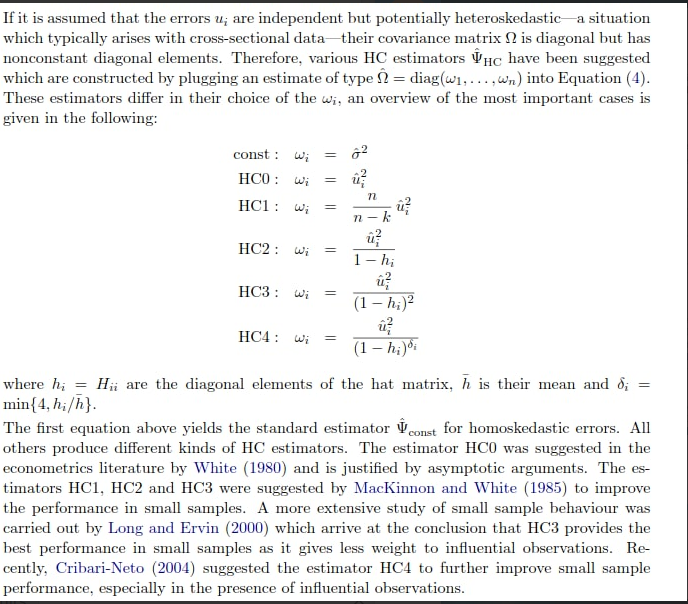
\includegraphics[width=0.7\linewidth]{screenshot011}
%	\caption{}
%	\label{fig:screenshot011}
%\end{figure}
%
%https://cran.r-project.org/web/packages/sandwich/vignettes/sandwich.pdf

\textit{Взвешенный метод наименьших квадратов: }

$$
Y_{i}=\beta_{0}+\beta_{1} X_{i}+u_{i}
$$
Пусть
$$
\operatorname{var}\left(u_{i} \mid X_{i}\right)=\lambda h\left(X_{i}\right)
$$
где $\lambda$ -некоторая константа, $h\left(X_{i}\right)$ - известная функция.
Рассмотрим преобразованные переменные:
$$
\tilde{Y}_{i}=\frac{Y_{i}}{\sqrt{h\left(X_{i}\right)}} ; \tilde{X}_{0 i}=\frac{1}{\sqrt{h\left(X_{i}\right)}} ; \tilde{X}_{1 i}=\frac{X_{i}}{\sqrt{h\left(X_{i}\right)}} ; \text { и } \tilde{u}_{i}=\frac{u_{i}}{\sqrt{h\left(X_{i}\right)}}
$$

Тогда (1) примет вид
$$
\tilde{Y}_{i}=\beta_{0} \tilde{X}_{0 i}+\beta_{1} \tilde{X}_{1 i}+\tilde{u}_{i}
$$
$\hat{\beta}_{1}$ - ВМНК-оценка коэффициента наклона в уравнении (1) и она ВLUE

Заметим, что
$$
\begin{array}{l}
\operatorname{var}\left(\tilde{u}_{i} \mid X_{i}\right)=\operatorname{var}\left(\frac{u_{i}}{\sqrt{h\left(X_{i}\right)}} \mid X_{i}\right)= \\
=\frac{\operatorname{var}\left(u_{i} \mid X_{i}\right)}{h\left(X_{i}\right)}=\frac{\lambda h\left(X_{i}\right)}{h\left(X_{i}\right)}=\lambda=\text { const }
\end{array}
$$
HO!
$h\left(X_{i}\right)$ - в реальной жизни неизвестна $\rightarrow$ такая оценка называется недоступной ВМНК - оценкой


Доступный ВМНК - алгоритм: 

\begin{enumerate}
	\item Оцените регрессию (1) на при помощи МНК и вычислите остатки $\hat{u}_{i}, i=1, \ldots, n$
\item  Оцените предполагаемую модель функции условной дисперсии $\operatorname{var}\left(u_{i} \mid X_{i}\right)$ (оцениваем $\hat{u}_{i}^{2}$ на набор переменных, от которых она зависит).
\item  Используйте оцененную функцию для расчета предсказанных значений функции условной дисперсии $\widehat{\operatorname{var}}\left(u_{i} \mid X_{i}\right)$
\item  Умножьте зависимую переменную и регрессоры (в том числе и свободный член) на величину, обратную квадратному корню из оцененной функции условной дисперсии (см. (2)).
\item  Оцените коэффициенты взвешенной регрессии (3) при помощи МНК; полученные оценки являются ВМНК-оценками (1).
\end{enumerate}


\textit{ВМНК или устойчивые к гетероскедастичности
стандартные ошибки: }

\begin{enumerate}
	\item ВМНК:
	\begin{itemize}
		\item «+» более эффективные, чем МНК, оценки коэффициентов с использованием сырых
	(не скорректированных) регрессоров;
	\item  «-» необходимо знать функцию условной дисперсии и оценки ее параметров, что
	может быть затруднительно на практике;
	\item  «-» если функциональная форма дисперсии неверна, то ВМНК с.о. регрессии
	являются неверными в том смысле, что они приводят к неправильным
	статистическим выводам;
	\end{itemize}
	\item  Устойчивые к гетероскедастичности с.о.:
	\begin{itemize}
		\item «+» асимптотически верные выводы, даже если вид функции условной дисперсии
	неизвестен;
	\item  «+» легко вычисляются;
	\item  «-» не эффективные по сравнению с ВМНК–оценкой (полученной на основе верной
	функции условной дисперсии), по крайней мере, асимптотически.
	\end{itemize}
\end{enumerate}

%\begin{figure}
%	\centering
%	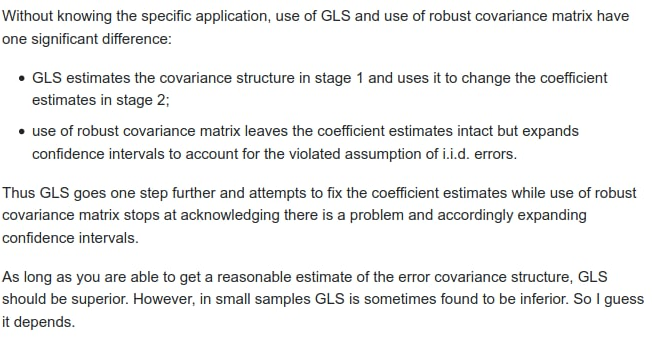
\includegraphics[width=0.7\linewidth]{screenshot012}
%	\caption{}
%	\label{fig:screenshot012}
%\end{figure}
%

Обобщенный метод наименьших квадратов: 

Generalized Least Square (GLS)
So far, we have been dealing with heteroskedasticity under OLS framework. But if we knew the variance-covariance matrix of the error term, then we can make a heteroskedastic model into a homoskedastic model.
As we defined before
$$
E\left(u u^{\prime}\right)=\sigma^{2} \Omega=\Sigma
$$
Define further that
$$
\Omega^{-1}=P^{\prime} P
$$
$P$ is a "n x n" matrix
Pre-multiply $P$ on a regression model
$$
P y=P X \beta+P u
$$
or
$$
\tilde{y}=\tilde{X} \beta+\tilde{u}
$$
In this model, the variance of $\tilde{u}$ is
$$
E\left(\tilde{u} \tilde{u}^{\prime}\right)=E\left(P u u^{\prime} P^{\prime}\right)=P E\left(u u^{\prime}\right) P^{\prime}=P \sigma^{2} \Omega P^{\prime}=\sigma^{2} P \Omega P^{\prime}=\sigma^{2} I
$$
Note that $P \Omega P^{\prime}=I,$ because define $P \Omega P^{\prime}=A,$ then $P^{\prime} P \Omega P^{\prime}=P^{\prime} A .$ By the definition of $P, \Omega^{-1} \Omega P^{\prime}=P^{\prime} A,$ thus $P^{\prime}=P^{\prime} A .$ Therefore, $\boldsymbol{A}$ must be $\boldsymbol{I} .$

Weighted Least Squares Estimation (WLS)
Consider a general case of heteroskedasticity.
$$
\operatorname{Var}\left(u_{i}\right)=\sigma_{t}^{2}=\sigma^{2} \omega_{i}
$$
Then,
$$
E\left(u u^{\prime}\right)=\sigma^{2}\left[\begin{array}{ccc}
\omega_{1} & 0 & 0 \\
0 & \omega_{2} & 0 \\
0 & 0 & \omega_{u}
\end{array}\right]=\sigma^{2} \Omega, \text { thus } \Omega^{-1}=\left[\begin{array}{ccc}
\omega_{1}^{-1} & 0 & 0 \\
0 & \omega_{2}^{-1} & 0 \\
0 & 0 & \omega_{n}^{-1}
\end{array}\right]
$$


\textit{Тестирование гетероскедастичности: }

\begin{itemize}
	\item Графические методы: график остатков модели $\hat{u}_{i}$, 
	график стандартизованных остатков $c_{i}=\frac{\widehat{u}_{i}}{s_{\widehat{u}}}$
	от 
	\begin{itemize}
		\item 	оцененных значений $\hat{y}_{i}$: позволяют выявить выбросы, возможную гетероскедастичность, неправильную спецификацию модели;
		\item  отдельных объясняющих переменных: позволяют выявить возможную нелинейность;
		\item  номера наблюдения (последовательные моменты времени):  позволяют выявить изменение дисперсии ошибок во времени, пропуск переменных, автокоррелированность ошибок.
	\end{itemize}
	\item Формальные процедуры: тесты  Голдфелда-Квандта (Goldfeld-Quandt),  Глейзера  (Glejser),  Бройша-Пагана  (Breusch-Pagan).  
\end{itemize}

\textit{Тесты  Голдфелда-Квандта (Goldfeld-Quandt) }

\begin{enumerate}
	\item Упорядочиваем наблюдения по предполагаемому возрастанию дисперсий ошибок (по предполагаемой переменной);
	\item  Отбрасываем $r$ центральных наблюдений;
	\item  Оцениваем выбранную модель отдельно на первом и последнем интервале;
	\item  Вычисляем $F^{a c t}=\frac{R S S_{2}}{R S S_{1}} ;$
	\item  Гипотеза
	$H_{0}: \operatorname{var}\left(u_{i} \mid X_{i}\right)=\mathrm{const}, i=1, n$ (гомоскедастичность)
	отвергается, если $F^{a c t}>F_{1-\alpha}\left(\frac{n-r}{2}-2 ; \frac{n-r}{2}-2\right)$
\end{enumerate}

%\begin{figure}
%	\centering
%	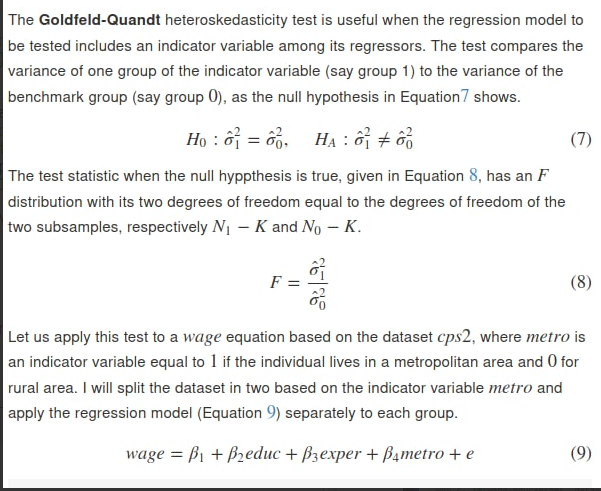
\includegraphics[width=0.7\linewidth]{screenshot015}
%	\caption{}
%	\label{fig:screenshot015}
%\end{figure}


\textit{Тест Глейзера  (Glejser)}

$$
\operatorname{var}\left(u_{i} \mid X_{i}\right)=\theta_{0}+\theta_{1} X_{i}^{\gamma}
$$
\begin{enumerate}
	\item Оцените регрессию (1) на при помощи МНК и вычислите остатки $\hat{u}_{i}, i=1, \ldots, n$
	\item Оцените регрессию $\left|\hat{u}_{i}\right|$ на константу и $X_{i}^{\gamma}$, специфицировав $\gamma .$ (Выбрав модель с самым высоким  $R^2$. Обычно $\gamma=1$, $\gamma=-1$, $\gamma=0.5$)
	\item  $H_{0}: \quad \theta_{1}=0, H_{1}: \quad \theta_{1} \neq 0$
	\item  Отвергаем $H_{0}$ на 5\% ур.зн., если $\left|t^{a c t}\right|>1,96$
\end{enumerate}

%\begin{figure}[H]
%	\centering
%	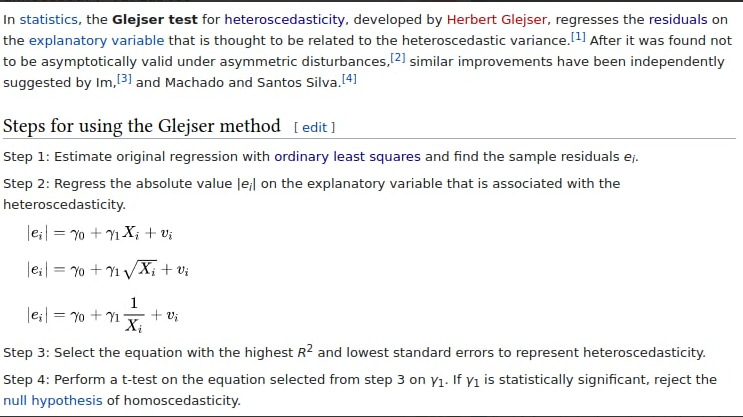
\includegraphics[width=0.7\linewidth]{screenshot005}
%	\caption{}
%	\label{fig:screenshot006}
%\end{figure}


\textit{Тест Бройша-Пагана  (Breusch-Pagan)}

Тест Бреуша - Пагана Тестируемая гипотеза в данном тесте состоит в том, что гетероскедастичности в модели нет:
$$
H_{0}: \sigma_{1}^{2}=\ldots=\sigma_{n}^{2}
$$

Тест Бреуша - Пагана Тестируемая гипотеза в данном тесте состоит в том, что гетероскедастичности в модели нет:
$$
H_{0}: \sigma_{1}^{2}=\ldots=\sigma_{n}^{2}
$$

Процедура осуществления теста устроена так: сначала при помощи обычного МНК оценивается исходная модель (для которой мы хотим проверить отсутствие гетероскедастичности) и вычисляются соответствующие остатки $e_{i} .$ Далее вычисляется вспомогательное значение $\tilde{\sigma}^{2}=\frac{1}{n} \sum e_{i}^{2} .$ После этого необходимо оценить вспомогательное уравнение, в котором справа стоят переменные, потенциально влияющие на дисперсию случайной ошибки:
$$
\frac{e_{i}^{2}}{\tilde{\sigma}^{2}}=\gamma_{0}+\gamma_{1} z_{i}^{(1)}+\ldots+\gamma_{p} z_{i}^{(p)}+u_{i}
$$
Далее вычисляется расчетное значение тестовой статистики по формуле:
$ESS/2$

Если верна нулевая гипотеза, то указанная статистика асимптотически имеет распределение Хи-квадрат с $p$ степенями свободы. Поэтому, если расчетное значение больше критического значения, взятого из таблиц распределения $\chi^{2}$ с $p$ степенями свободы для выбранного исследователем уровня значимости, то следует отвергнуть нулевую гипотезу и заключить, что в данных есть гетероскедастичность (необходимые таблицы доступны, например, в приложении к гл. 6). В противном случае можно сделать вывод в пользу гомоскедастичности.


%
%
%\begin{figure}[H]
%	\centering
%	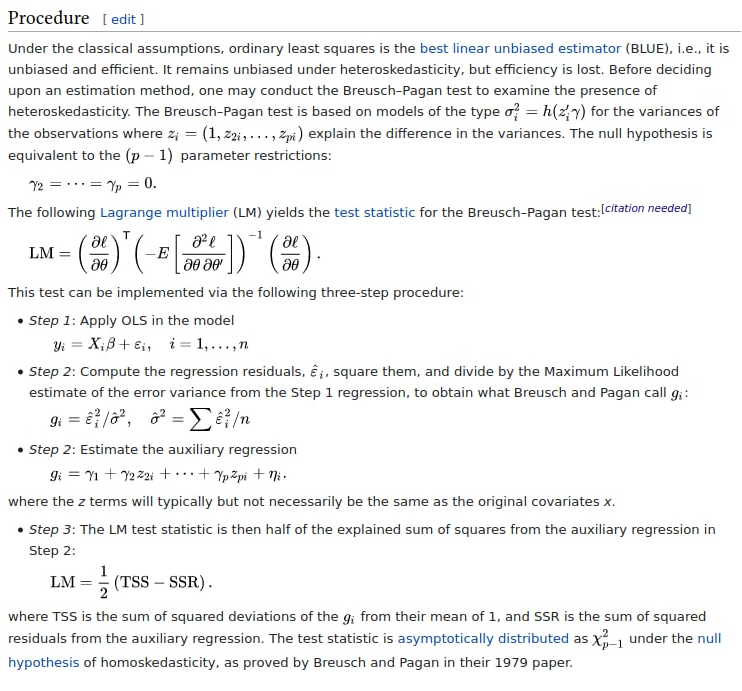
\includegraphics[width=0.7\linewidth]{screenshot006}
%	\caption{}
%	\label{fig:screenshot006}
%\end{figure}
%
%\begin{figure}
%	\centering
%	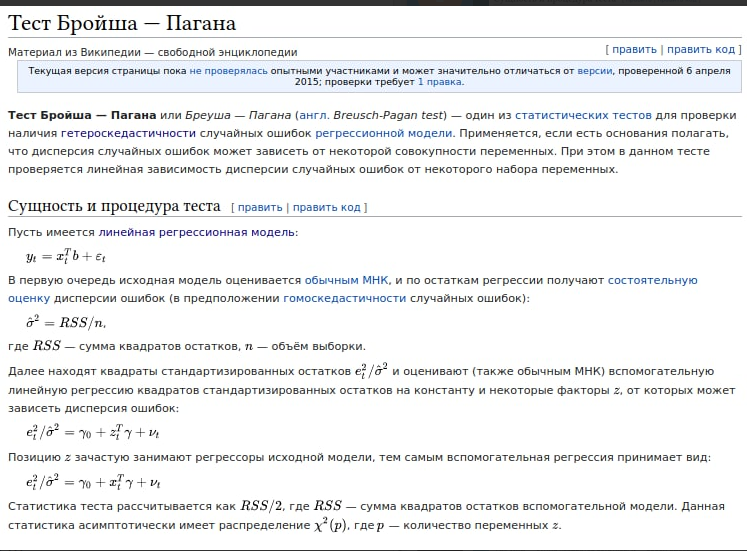
\includegraphics[width=0.7\linewidth]{screenshot013}
%	\caption{}
%	\label{fig:screenshot013}
%\end{figure}
%
%
%\begin{figure}
%	\centering
%	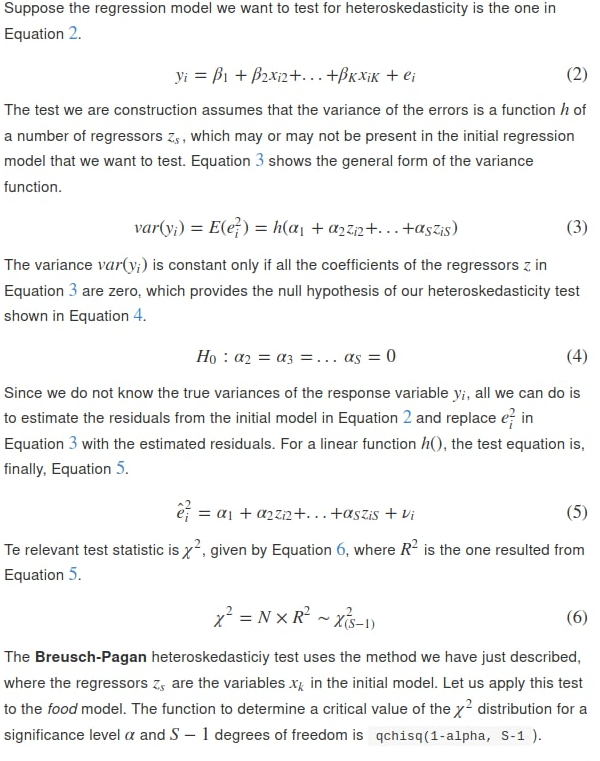
\includegraphics[width=0.7\linewidth]{screenshot014}
%	\caption{}
%	\label{fig:screenshot014}
%\end{figure}
%
%


%https://bookdown.org/ccolonescu/RPoE4/heteroskedasticity.html

\newpage



\textbf{Тема 5. Стохастические регрессоры. Эндогенность. Инструментальные переменные}

Предпосылки линейной модели со стохастическим регрессором (случай парной регрессии):
1. Модель линейна по параметрам и правильно специфицирована:
$$
y_{i}=\beta_{1}+\beta_{2} x_{i}+\varepsilon_{i}, \quad i=1,2, \ldots, n
$$
2. Наблюдения $\left\{\left(x_{i}, y_{i}\right), i=1, \ldots, n\right\}$ независимы и одинаково распределень.
3. $x_{i}$ и $y_{i}$ имеют ненулевые конечные четвертые моменты распределения $E\left(x_{i}^{4}\right)<\infty, \quad E\left(y_{i}^{4}\right)<\infty$
4. Случайные ошибки имеют нулевое условное математическое ожидание при заданном $x: E\left(\varepsilon_{i} \mid x_{i}\right)=0 .$


$$
Y_{i}=\beta_{0}+\beta_{1} X_{i}+\varepsilon_{i} \equiv \alpha+\beta_{1}\left(X_{i}-\bar{X}\right) i=1,2, \ldots, n
$$
Assumptions:
\begin{itemize}
	\item  $\left\{X_{i}, Y_{i}\right\}(i=1,2, \ldots, n)$ are $IID$ pairs, with $\operatorname{cov}\left(X_{i}, Y_{i}\right) \geq 0, \operatorname{var}\left(X_{i}\right)=\sigma_{X}^{2}>0$
$\operatorname{var}\left(Y_{i}\right)=\sigma_{Y}^{2}>0 \forall i$
\item  $  E\left(\varepsilon_{i} \mid X_{h}\right)=0, \forall i \text { and } h $
\item  $\operatorname{var}\left(\varepsilon_{i} \mid X_{h}\right)=\sigma^{2}, \forall i$ and $h$ and finite 4 th moments (no excess kurtosis)
\item  $\operatorname{cov}\left(\varepsilon_{i}, \varepsilon_{j} \mid X_{h}\right)=0, \forall i \neq j,$ and for all $h$
\item  $\beta_{0}, \beta_{1}$ and $\sigma^{2}$ are constant parameters
\item For the purpose of statistical inference in small samples we may invoke normally distributed disturbances:
$ \varepsilon_{i} \sim \operatorname{lIN}\left(0, \sigma^{2} \mid X_{h}\right) \text { . }
$
\end{itemize}



%\begin{figure}
%	\centering
%	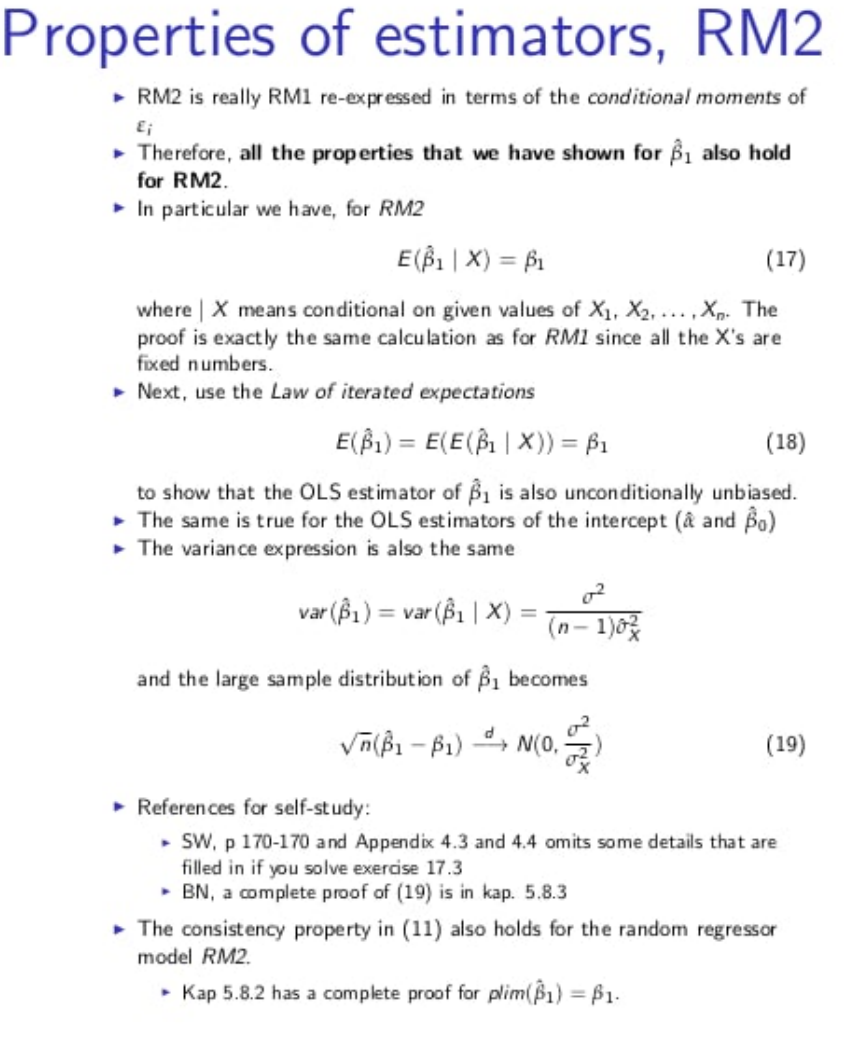
\includegraphics[width=0.7\linewidth]{screenshot018}
%	\caption{}
%	\label{fig:screenshot018}
%\end{figure}


Обобщение теоремы Гаусса-Маркова  на  случай  стохастических  регрессоров  (без  доказательства).  

THE EXTENDED LEAST SQUARES ASSUMPTIONS IN THE MULTIPLE REGRESSION MODEL
The linear regression model with multiple regressors is
$$
Y_{1}=X_{i}^{\prime} \beta+u_{i}, i=1, \ldots, n
$$
The extended least squares assumptions are

1. $E\left(u_{i} \mid X_{i}\right)=0$ (u, has conditional mean zero):

2. $\left(X, Y_{j}\right), i=1 \ldots \ldots n$ are independently and identically distributed (i.i.d.) draws from their joint distribution:

3. $X_{i}$ and $u_{i}$ have nonzere finite fourth moments:

4. $X$ has full column rank (there is no perfect multicollinearity):

5. $\operatorname{var}\left(u_{i} \mid X_{i}\right)=\sigma_{u}^{2}$ (homoskedasticity): and

6. the conditional distribution of $u_{i}$ given $X_{i}$ is normal (normal errors).


The Ganss-Markov conditions for multiple regression are

(i) $E(\boldsymbol{U} \mid \boldsymbol{X})=\boldsymbol{0}_{\boldsymbol{m}}$

(ii) $E\left(U U^{*} \mid X\right)=\sigma_{u}^{2} I_{n}$, and

(iii) $X$ has full column rank.

The Ganss-Markov conditions for multiple regression are
(i) $E(\boldsymbol{U} \mid \boldsymbol{X})=\boldsymbol{0}_{\boldsymbol{m}}$
(ii) $E\left(U U^{*} \mid X\right)=\sigma_{u}^{2} I_{n}$, and
(iii) $X$ has full column rank.

Suppose that the Gauss-Markov conditions for multiple regression in Equation (18.38) hold. Then the OL.S cstimator $\vec{\beta}$ is BLUE. That is, let $\bar{\beta}$ be a linear conditionally unbiascd estimator of $\beta$ and let $c$ be a nonrandom $k+1$ dimensional vector. Then $\operatorname{var}\left(\boldsymbol{c}^{\prime} \boldsymbol{\beta} \mid X\right) \leq \operatorname{var}\left(\boldsymbol{c}^{\prime} \boldsymbol{\beta} \mid X\right)$ for every nonzero vector $c$. where the
inequality holds with cquality for all c only if $\bar{\beta}=\hat{\beta}$.




Угрозы для внутренней
обоснованности

1. пропущенные переменные,

2. неправильная спецификация функциональной формы регрессии,

3. неточное измерение независимых переменных («ошибки в переменных»),

4. отбор наблюдений,

5. одновременная причинность.

Напомним, что в предыдущей главе мы сформулировали два важных определения:

- Эндогенный регрессор - это регрессор, который коррелирован со случайными ошибками модели: $\operatorname{cov}\left(x_{i}, \varepsilon_{i}\right) \neq 0 .$

- Экзогенный регрессор - это регрессор, который не коррелирован со случайными ошибками модели: $\operatorname{cov}\left(x_{i}, \varepsilon_{i}\right)=0 .$

Могут возни-
кать следующие типичные ситуации:

1. Эндогенность регрессора из-за пропуска существенной перемен-
ной. В качестве важного частного случая тут также следует ука-
зать проблему эндогенности из-за самоотбора.

2. Эндогенность регрессора из-за выбора неверной функциональ-
ной формы связи.

3. Эндогенность регрессора из-за двусторонней причинно-следст-
венной связи.

4. Эндогенность регрессора из-за ошибок измерения.

Проблема  эндогенности.



Метод инструментальных переменных (instrumental variables, IV). 

Представим, что в нашем распоряжении кроме информации о переменных $x$ и $y$ есть еще данные о третьей переменной $z,$ которая удовлетворяет двум свойствам:

- релевантность (relevance): $\operatorname{cov}\left(z_{i}, x_{i}\right) \neq 0 ;$

- экзогенность (exogeneity): $\operatorname{cov}\left(z_{i}, \varepsilon_{i}\right)=0 .$

Первый шаг Оцениваем регрессию переменной $x$ по переменной z:

$$
\hat{x}_{i}=\hat{\theta}_{1}+\hat{\theta}_{2} z_{i}
$$

Получаем прогнозные значения $\hat{x}_{i}$

Второй Шаг Оцениваем регрессию переменной $y$ по этим предсказанным значениям $\hat{x}:$
$$
\hat{y}_{i}=\hat{\beta}_{1}+\hat{\beta}_{2} \hat{x}_{i}
$$
Чтобы отличать оценку коэффициента, полученную таким способом, от обычной МНК-оценки, мы иногда будем использовать в обозначени и дополнительный индекс: $\beta_{2}^{\text {TSLS }}$


$$
\hat{\beta}_{2}^{\mathrm{TSLS}}=\frac{\frac{1}{n} \Sigma\left(y_{i}-\bar{y}\right)\left(z_{i}-\bar{z}\right)}{\frac{1}{n} \Sigma\left(x_{i}-\bar{x}\right)\left(z_{i}-\bar{z}\right)}=\frac{\widehat{\operatorname{cov}(y, z)}}{\widehat{\operatorname{cov}(x, z)}}
$$


Для случая гомоскедастичности корректная формула стандартной ошибки коэффициента при регрессоре имеет
$$
\operatorname{se}\left(\hat{\beta}_{2}\right)=\sqrt{\frac{S^{2}}{\sum\left(x_{i}-\bar{x}\right)^{2}} \cdot \frac{1}{\operatorname{corr}^{2}(x, z)}}, \quad S^{2}=\frac{\sum_{i=1}^{n} e_{i}^{2}}{n-2}
$$


Векторно-матричная форма записи

$$
y_{i}=\beta_{0}+\beta_{1} \cdot x_{i}^{(1)}+\ldots+\beta_{p} x_{i}^{(p)}+\beta_{p+1} w_{i}^{(1)}+\ldots+\beta_{p+r} w_{i}^{(r)}+\varepsilon_{i}
$$

$y=X \beta+\varepsilon$


На первом шаге двухшагового МНК мы оцениваем регрессию $X$ по $Z .$ Это можно записать так:
$$
\hat{X}=Z \hat{\alpha} .
$$
По формуле для МНК-оценки из $\S 3.3 \hat{\alpha}=\left(Z^{\prime} Z\right)^{-1} Z^{\prime} X,$ следовательно:
$$
\hat{X}=Z\left(Z^{\prime} Z\right)^{-1} Z^{\prime} X
$$
На втором шаге двухшагового МНК мы оцениваем регрессию $y$ по $\hat{X}:$
$$
\hat{y}=\hat{X} \hat{\beta}^{\mathrm{TSLS}}
$$

Таким образом, окончательно имеем следующую формулу для 2МНК-оценки:
$$
\hat{\beta}^{\mathrm{TSLS}}=\left(X^{\prime} Z\left(Z^{\prime} Z\right)^{-1} Z^{\prime} X\right)^{-1} X^{\prime} Z(Z Z)^{-1} Z^{\prime} y .
$$


Если число инструментов в точности совпадает с числом эндогенных регрессоров $(m=p),$ то матрицы $X$ и $Z$ имеют одинаковую размерность. В этом случае выражение для оценки $\hat{\beta}^{\text {TSLS }}$ можно упростить:

$\hat{\beta}^{\mathrm{IV}}=\left(Z^{\prime} X\right)^{-1} Z^{\prime} y$


%\begin{figure} [H]
%	\centering
%	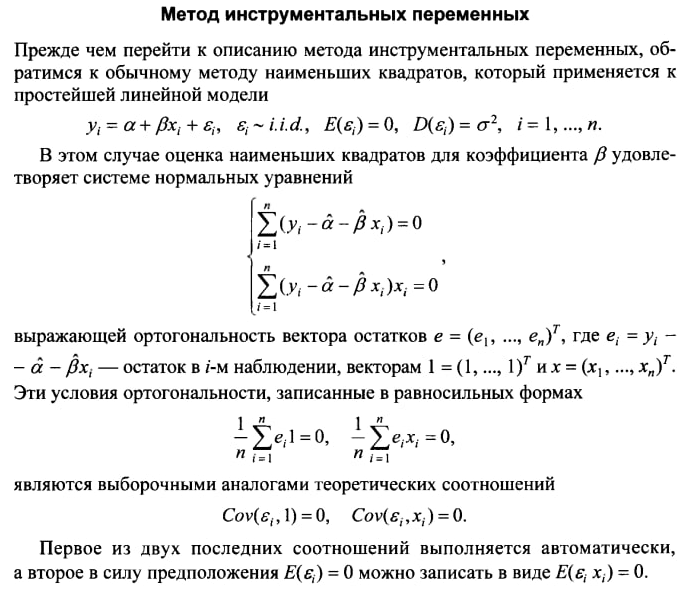
\includegraphics[width=0.7\linewidth]{screenshot019}
%	\caption{}
%	\label{fig:screenshot019}
%\end{figure}
%
%
%\begin{figure}[H]
%	\centering
%	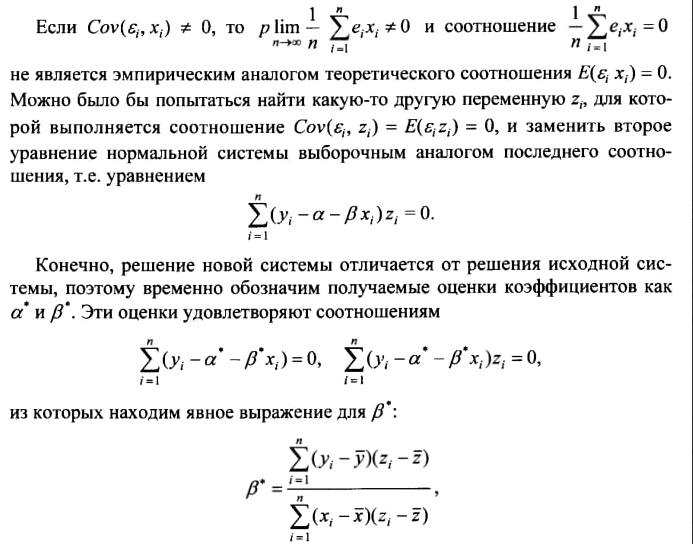
\includegraphics[width=0.7\linewidth]{screenshot020}
%	\caption{}
%	\label{fig:screenshot020}
%\end{figure}
%
%\begin{figure}[H]
%	\centering
%	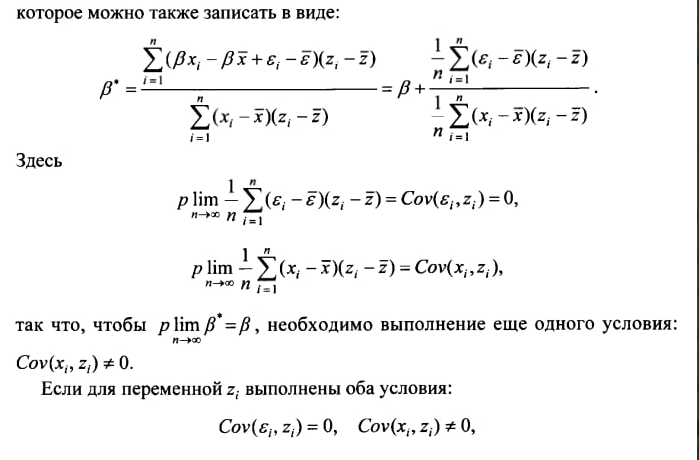
\includegraphics[width=0.7\linewidth]{screenshot021}
%	\caption{}
%	\label{fig:screenshot021}
%\end{figure}
%
%\begin{figure}[H]
%	\centering
%	
\includegraphics[width=0.7\linewidth]{screenshot022}
%	\caption{}
%	\label{fig:screenshot022}
%\end{figure}
%
%\begin{figure}[H]
%	\centering
%	
\includegraphics[width=0.7\linewidth]{screenshot023}
%	\caption{}
%	\label{fig:screenshot023}
%\end{figure}
%
%
%\begin{figure}[H]
%	\centering
%	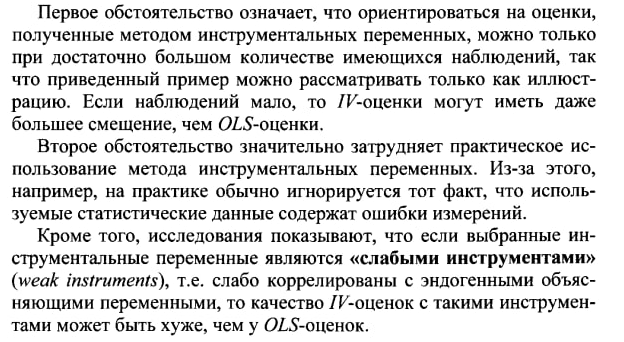
\includegraphics[width=0.7\linewidth]{screenshot024}
%	\caption{}
%	\label{fig:screenshot024}
%\end{figure}
%


\textit{Обобщенный метод моментов}

\url{http://www.eco.uc3m.es/~ricmora/mei/materials/Session_12_GMM.pdf}

\newpage

\textbf{Тема 6. Системы одновременных уравнений}


Структурная форма системы одновременных уравнений -  в явном виде представлены взаимные связи между
входящими в модель переменными

\begin{equation*} 
\begin{cases}
C_t = \alpha + \beta Y_t + \epsilon_t \\
Y_t = C_t + I_t 
\end{cases}
\end{equation*}


Приведенная форму системы одновременных уравнений - выраженные из системы объясняемые перемненные (взаимодействие между перменными  представлено неявном, однако коэффициенты приведенной формы отражают итог взаимодействия этих переменных)

\begin{equation*} 
\begin{cases}
C_t = \frac{\alpha}{1-\beta} + \frac{\beta}{1-\beta}  I_t +  \frac{1}{1-\beta} \epsilon_t \\
Y_t = \frac{\alpha}{1-\beta}  + \frac{1}{1-\beta} I_t + \frac{1}{1-\beta} \epsilon_t  
\end{cases}
\end{equation*}


\textit{Идентифицируемость}

Структурное уравнение называется \textbf{идентифицируемым}, если его коэффициенты можно выразить через коэффициенты приведённой формы. Если это можно сделать единственным способом, то говорят о точной индентифицируемости, если несколькими способами — о \textbf{сверхидентифицируемости}. В противном случае оно называется неидентифицируемым. Сверхидентифицируемость фактически означает, что на коэффициенты приведённой формы наложены некоторые ограничения (сверхидентифицирующие). 

Cистема частично идентифицируема, если коэффициенты одного из уравнений восстанавливаются по коэффициентам приведенной формы. 


При рассмотрении условий идентифицируемости отдельных структурных
уравнений, предполагается, что переменные, задействованные в системе, подразделяются на три типа: 

- эндогенные переменные (эндогенная переменная, входящая в $i$-е уравнение системы, коррелирована с ошибкой в этом уравнении. )
- экзогенные переменные (экзогенные переменные не коррелированы с ошибками во всех уравнениях системы для всех моментов времени.)
- предопределенные переменные  (значение предопределенной переменной, входящей в уравнение, не должно быть коррелированным со значениями ошибки в этом уравнении, соответствующими моментам  $t, t + 1,... $  


Предполагается, что:

- система состоит из $g$ уравнений
- $g$ эндогенных переменных; $К$ экзогенных и предопределенных переменных;
- каждое из g уравнений нормировано (normalized), так что коэффициент при одной из эндогенных переменных, входящих в уравнение, равен 1.


Условие порядка  и  условие  ранга.  

Условия идентифицируемости отдельного структурного уравнения

Поскольку $ \Pi \Gamma = B  $ и мы использовали это соотношение для восстановления коэффициентов структурных уравнений двух последних систем, вопрос об идентифицируемости структурной формы — это вопрос о возможности однозначного восстановления всех коэффициентов структурной формы, т.е. восстановления матриц $Г$ и $В$, на основании матрицы $П= ВГ^{-1}$ . 

В совокупности матрицы  $Г$ и $В$ состоят из $g^2 + Kg$ элементов, тогда как в матрице П всего $Kg$ элементов. Поэтому однозначное восстановление коэффициентов структурной формы по коэффициентам приведенной формы невозможно без использования дополнительной информации в виде невключения в отдельные уравнения тех или иных переменных, нормировки коэффициентов, линейных
ограничений на параметры структуры.



Пусть матрица $А$ размера $(g + К) * g$ составлена из матриц $Г$ и $В$ таким образом, что матрица $Г$ располагается над матрицей $В$

Коэффициенты при $g$ эндогенных и $К$ предопределенных переменных в i-м
структурном уравнении составляют $i$-й столбец $а_i$, матрицы $A$.

Существенным является то обстоятельство, что коэффициенты $i$-го структурного уравнения не могут быть восстановлены на основании коэффициентов приведенной формы, если в это уравнение входят все $g + К$ переменные системы.
Поэтому далее будем предполагать, что на элементы вектора $а_i$, помимо
нормировочного накладываются еще и некоторые дополнительные однородные линейные ограничения в виде уравнений:

$\Phi_i a_i = 0 $

где $\Phi_i $ — матрица размера $R_i * (g+K) $, $R_i$ — количество линейных ограничений.


Пусть $А_i$ — матрица, получаемая из матрицы $А$ вычеркиванием ее $i$-го столбца так что $А = [а_i : А_i]$.

Тогда  $ rank (\Phi_i А) =  rank (\Phi_i a_i : \Phi_i А_i ) = rank (0  : \Phi_i А_i ) = rank (\Phi_i А_i ) $ 

Но матрица $\Phi_i А_i$    имеет размер $ R_i * (g - 1)$, и, чтобы ее ранг был равен $(g - 1)$, во всяком случае необходимо выполнение следующего порядкового условия идентифицируемости 



\textit{Необходимое условие идентифицируемости структурного уравнения (порядковое условие): }

Количество переменных правой части уравнения должно быть не больше количества всех экзогенных переменных системы. 

В канонической форме: количество исключенных из данного уравнения экзогенных переменных должно быть не меньше количества включенных эндогенных переменных уравнения минус единица. 

$$ R_i \geq g - 1 $$ 

\textit{Достаточное условие идентифицируемости структурного уравнения (ранговое условие):}


Ранг матрицы, составленной из коэффициентов (в других уравнениях) при переменных, отсутствующих в данном уравнении, не меньше общего числа эндогенных переменных системы минус единица:

$$ rank (\Phi_i A )  = g - 1 $$



- $ rank (\Phi_i A )  < g - 1 $ - уравнение неидентифицируемо
- $ rank (\Phi_i A )  = g - 1 $ и $ R_i = g - 1 $  уравнение идентифицируемо точно 
- $ rank (\Phi_i A )  =  g - 1 $  и $ R_i > g - 1 $  - уравнение сверхидентифицируемо


В ситуациях 2 и 3, если рассматривать задачу восстановления коэффициентов $i$-го структурного уравнения на
основании МНК-оценок коэффициентов приведенной формы  каждого отдельного уравнения приведенной системы, не учитывающим ограничения на коэффициенты приведенной формы, то по $\hat{\Pi}$  в ситуации 2  структурного уравнения восстанавливаются  однозначным образом, тогда как в ситуации 3 существует несколько вариантов восстановления.



Оценивание  систем  одновременных  уравнений.  



Идентифицируемость системы структурных уравнений в целом (на основании приведенной формы системы) означает идентифицируемость не только
всех коэффициентов системы, но и ковариационной матрицы случайных
ошибок, входящих в правые части уравнений системы. 

При этом при восстановлении коэффициентов и ковариационной матрицы ошибок в структурной форме используются не только коэффициенты приведенной формы, но и ковариационная матрица ошибок в приведенной форме.

Пусть $E(u_t) = 0, \Sigma =(  Cov(u_{it}, u_{tj} )) = (\sigma_{ij}) $ - диагональная матрица


Ошибки не коррелированы по времени, но для одного и того же момента
ошибки в разных уравнениях могут быть коррелированными между собой:

Тогда   $E(w_t) = 0, \Omega  =(  Cov(w_{it}, w_{tj} )) =   Cov(u_{t} \Gamma^{-1}  ) =  (\Gamma^{-1})^T \Sigma (\Gamma^{-1})  $ 

$$\Sigma = \Gamma^T \Sigma \Gamma $$

Следовательно, если структурная система идентифицируема (коэффициенты структурной системы однозначно восстанавливаются по коэффициентам
приведенной формы), то тогда, восстановив по коэффициентам приведенной
формы матрицу $Г$, можно, используя эти восстановленные коэффициенты
и матрицу $\Omega$, восстановить ковариационную матрицу $\Sigma$.

Если структурная форма не восстанавливается целиком, а возможно лишь
восстановление некоторых ее уравнений, то тогда для полной идентификации $i$-го стохастического структурного уравнения надо восстановить все его коэффициенты и дисперсию случайной составляющей этого уравнения. 


\textit{Рекурсивная  СОУ }

Рекурсивная система - благодаря последовательному определению эндогенных переменных в таких системах при переходе
от уравнения к уравнению, в правых частях каждого из уравнений
системы не оказывается переменных, значения которых коррелированы со значением ошибки в этом уравнении при одном и том же t.

\textit{Косвенный метод наименьших квадратов (ILS)}

Если $i$-е стохастическое уравнение структурной формы идентифицируемо
точно, то параметры этого уравнения (коэффициенты уравнения и дисперсия
случайной ошибки) восстанавливаются по параметрам приведенной системы
однозначно. Поэтому для оценивания параметров такого уравнения достаточно оценить коэффициенты каждого из уравнений приведенной формы
с помощью МНк (отдельно для каждого уравнения) и получить оценку ковариационной матрицы $\Sigma$ ошибок в приведенной форме, после
чего воспользоваться соотношениями $ПГ = В, \Sigma = \Gamma^T \Omega \Gamma $ по $\hat{\Pi}, \hat{\Omega}$ . 

Полученные в результате оценки коэффициентов $i$-го
стохастического уравнения структурной формы наследуют свойство состоятельности оценок приведенной формы. Однако они не наследуют таких
свойств оценок приведенной формы, как несмещенность и эффективность,
из-за того что получаются в результате нелинейных преобразований.


\textit{Двухшаговый метод наименьших квадратов (2SLS)}

Рассмотрим систему $g$ одновременных уравнений:

$$y_t \Gamma = x_t B + u_t$$ 

Считая, что первое уравнение нормировано на коэффициент при переменной $y_t1$, преобразуем уравнение к виду:

$$y_t1 \Gamma = \alpha_{11} y_{t1}^* + ... + \alpha_{g1}  y_{tg}^*  +    \theta_{11} x_{t1}^*  + ... + \theta_{K1} x_{tK}^*   + u_t1$$ 


Состоятельному оцениванию коэффициентов уравнения мешает эндогенность переменных $у^*_{t1}, ..., у^*_{tg_1} $ . 

1 шаг:


Производится оценивание уравнений регрессии каждой из этих переменных на все предопределенные переменные, включенные в систему.

$$Y_i = X \Pi_i + W_i$$ 

Оценив отдельные уравнения с помощью МНК, получим
оценку $\hat{П}_i $, матрицы ${П}_i $  и на ее основе — оценку матрицы $Y_i$, в виде $\hat{Y}_i = X \hat{П}_i  $

Матрица $\hat{Y}_i$, содержит значения эндогенных переменных, включенных в правую часть $i$-го структурного уравнения, «очищенных» от корреляции с ошибкой в этом уравнении.


2 шаг:

Значения эндогенных переменных в первом уравнении  $у^*_{t1}, ..., у^*_{tg_1} $  заменяются значениямиy  $\hat{у}^*_{t1}, ..., \hat{у}^*_{tg_1} $. Полученное уравнение оценивается МНК.

Запишем уравнение в виде:

$$y_i = Y_i \alpha_i + X_i \theta_i +u_i = \hat{Y}_i    \alpha_i + X_i \theta_i +  \epsilon_i = \hat{Z}_i \delta_i +  \epsilon_i $$

где $ \epsilon_i = ( Y_i - \hat{Y}_i  )  \alpha_i  +   u_i $


Вычислим МНК-оценки  вектора $\delta_i $: 

$$ \hat{\delta}_i^{2SLS} = (\hat{Z}_i^T \hat{Z}_i )^{-1} \hat{Z}_i^T y_i $$ 


Для состоятельности  $ \delta_i^{2SLS}$ требуется еще, чтобы предельная матрица имела конечные элементы и была невырожденной, а для этого матрица $П_i$  должна иметь полный столбцовый ранг. 

$$ p \lim_{n\to \infty} (\frac{1}{n} \hat{Z}_i^T \hat{Z}_i ) = Q_i $$ 


Для построения t-статистик и доверительных интервалов, значения стандартных ошибок коэффициентов должны быть скорректированы


Проверка адекватности

Применив 2SLS  к i-му структурному уравнению, получим вектор остатков $  \hat{u_i} ^{2SLS} = y_i -   \hat{y}_i^{2SLS}$, опираясь на который  можно обычным образом проверять адекватность уравнения, используя
критерии:
- нормальности (Харке — Бера);
- линейности (добавляя степени и перекрестные произведения предопределенных переменных)
- гомоскедастичности (Уайта, Пагана — Холла для выявления гетероскедастичности в отдельном уравнении системы);
- автокоррелированности остатков (Бройша — Годфри)




\textbf{Тема 7. Бинарные объясняемые переменные. Логит и пробит модели} 

Классическая линейная модель:

$$y_i = \theta_1 x_{i1} + ... + \theta_p x_{ip} + u_i$$


Попытка оценить такую модель МНК наталкивается на определенные трудности: 

При обычном предположении:
$$ E(y_i | х_i) = x_i^T \theta $$


В то же время, поскольку $y_i$  принимает только значения — 0 и 1, ее условное математическое ожидание (при заданном
значении х,) равно:

$$ E(y_i | х_i)   =   Р \{ у_i  = 1| х_i  \} $$  


Таким образом $$ x_i^T \theta =  Р \{ у_i  = 1| х_i  \} $$ - вероятность, а значит, она должна быть в рамках $[0,1]$ 

$$Var(\epsilon_i|x_i) = x_i^T\theta(1-x_i^T\theta)$$

Также возникает проблема гетероскедастичности,
осложненная еще и тем, что в выражения для дисперсий
входит (неизвестный) вектор параметров $\theta$.


Коэффициент $\theta$ практически всегда   является неинтерпретируемым. 


Логит-, пробит-, гомпит-модели


$$ у_i = G(\theta_1 x_{i1} + ... + \theta_p x_{ip} ) + u_i =  G(x_{i}^T \theta) + u_i $$


Предположим, что при фиксированных значениях объясняющих переменных, случайные ошибки статистически независимы, так что функция правдоподобия параметров имеет вид:

$$ L(\theta|x) = \prod  (G(x_{i}^T \theta))^{y_i} (1- G(x_{i}^T \theta))^{1 - y_i} $$


Максимизируя логарифмическую функцию правдоподобия, получаем оценки $\hat{\theta}$. 


- Пробит-модель - функция стандартного нормального распределения

$$\Phi (z) = \frac{1}{\sqrt{2\pi}} \int_{-\infty}^{z} e^{-t^2/2}dt  $$

- Логит-модель - функция стандартного логистического распределения

$$\Lambda (z) = \frac{e^z}{1+e^z}$$

- Гомпит-модель - функция стандартного распределения экстремальных значений (минимума) I типа (распределение Гомпертца)

$$ G(z) = 1 -exp(-e^z)$$





\textit{Интерпретация коэффициентов}

Поскольку модели логит, пробит и гомпит являются нелинейными, оцененные коэффициенты в этих моделях имеют интерпретацию, отличающуюся
от интерпретации коэффициентов в линейной модели.


Пусть $k$-я объясняющая переменная является непрерывной переменной.
Тогда предельный эффект (marginal effect) этой переменной определяется
как производная:

$$\frac{\partial P\{ y_i = 1| x_i\}}{\partial x_{ik}} = \frac{\partial G (x_i^T \theta )}{\partial x_{ik}}$$

и в отличие от линейной модели этот эффект зависит от значений объясняющих переменных для $i$-го субъекта. 


$$\Delta P\{ y_i = 1| x_i\}  = \frac{\partial P\{ y_i = 1| x_i\}}{\partial x_{ik}} \Delta x_{ik} = \frac{\partial G (x_i^T \theta )}{\partial x_{ik}} \Delta x_{ik}$$

В случае когда сама объясняющая переменная - дамми-переменная, предельный эффект определяют просто как разность

$$\Delta P\{ y_i = 1| x_i, d_i=1\} - \Delta P\{ y_i = 1| x_i, d_i=0\} $$



Пусть $р$ — вероятность некоторого события. Отношение шансов $\frac{p}{1-p}$


Логарифм отношения шансов называют логитом: $logit(р) = \ln  \frac{p}{1-p}$ 


Если  $logit(p) > 0$, то больше шансов, что событие А произойдет. Если $logit(p) < 0$, то больше шансов, что событие А не произойдет.


Логит-модель линейна в отношении логита. Отсюда вытекает, что изменение значения $k$-й объясняющей переменной на величину $\Delta x_{ik}$ приводит (при неизменных значениях остальных объясняющих переменных) к изменению значения логита на $\theta_k \Delta x_{ik} $


\textit{ROC –кривая.}

\url{https://developers.google.com/machine-learning/crash-course/classification/roc-and-auc}

\newpage

\textbf{Тема 8. Модели панельных данных} 

Панельные данные (panel data) - данные о значениях переменных $у$ и $х$ для $N$ субъектов в $T$ последовательных моментов времени.

$$\{ у_{it}, х_{it}; i = 1, \dots, N, t = 1, \dots, T) \} $$


В общем случае $х$ является вектором конечной размерности $р$, и наиболее общей формой линейной модели наблюдений для
такой ситуации являлась бы спецификация 

$$y_{it} =x_{it}^u + \theta_{it} + u_{it} $$

где $\theta_{it}$ измеряет частное влияние $x_{it}$ в момент  $t$ для субъекта $i$.


\textit{Модели  сквозной  регрессии.  }

Модель пула ($ \theta_{it} = \theta $ ) :

$$ y_{it} = x_{it}^T \theta + u_{it} $$ 

в которой предполагается, что
$$u_{it} \sim i.i.d, \ E(x_{it}u_{js}) = 0 \ for  \  \forall  \ i,j = 1,\dots, N, \  t, s = 1, ..., T$$
так что $х$ является экзогенной переменной. 

В этом случае имеем дело с обычной линейной регрессией с $NT$ наблюдениями, удовлетворяющей предположениям классической нормальной линейной модели. 

Эффективные оценки параметров модели пула:  

Для получения эффективных оценок вектора коэффициентов в достаточно использовать обычный метод наименьших квадратов (OLS). При соответствующих предположениях о поведении значений объясняющих переменных, когда $N \to \infty$  или $Т \to \infty $,
эта оценка является также состоятельной оценкой этого вектора.



\textit{Модели  с  фиксированными эффектами. }

Обратимся теперь к методам анализа панельных данных, предназначенным
в основном для анализа данных, в которых
количество субъектов исследования $N$ велико, а количество наблюдений $Т$ над каждым субъектом мало. 


Модели со скалярной объясняющей переменной $х$

$$ y_{it} = \alpha_i + \beta x_{it} + u_{it} $$

равносильна

$$ y_{it}  = \sum \alpha_i d_{ij} + \beta x_{it}+ u_{it}$$ 

где $d_{ij} = 1$, если $j = i$

Здесь $\alpha_i$ -  неизвестные фиксированные  эффекты. 



$u_{it} \sim N(0, \sigma^2_u), \  E(x_{it}u_{js}) = 0 \ для \ \forall  i , j = 1, ..., N, \ t, s = 1, ..., T $ 

так что х является экзогенной переменной.




Модели с фиксированными эффектами наиболее подходят для случаев, когда субъектами исследования выступают страны, крупные компании или предприятия. Эти эффекты по существу, отражают наличие у субъектов индивидуальных характеристик, не изменяющихся со временем в процессе наблюдений, которые трудно или даже невозможно наблюдать или измерить.
Если значения таких характеристик не наблюдаются,
то эти характеристики невозможно непосредственно включить в правые
части уравнений регрессии в качестве объясняющих переменных, тогда
чтобы исключить смещение оценок из-за «пропущенных переменных», в правые части уравнений вместо значений ненаблюдаемых индивидуальных характеристик как раз и вводятся ненаблюдаемые эффекты $\alpha_i$. 


FE-оценка (within-estimator)

Оценки для фиксированных эффектов вычисляются по формуле:

$$\hat{\alpha}_i = \bar{y}_i - \hat{\beta} \bar{x}_i $$

OLS-оценка имеет вид:


$$\hat{\beta}_{CV} = \frac{\sum(x_{it} - \bar{x}_i)(y_{it} - \bar{y}_i)}{\sum (x_{it} - \bar{x}_i)^2 }$$


$$Var(\hat{\beta}_{CV}) = \frac{ \sigma^2_u }{\sum (x_{it} - \bar{x}_i)^2 }$$


Оценка имеет одно и то же значение как в рамках статистической
модели с дамми-переменными

$$ y_{it}  = \sum \alpha_i d_{ij} + \beta x_{it}+ u_{it}$$ 

и в рамках модели отклонения от групповых средних 

$$y_{it} - \bar{y}_i = \beta (x_{it} - \bar{x}_i )  + (u_{it} - \bar{u}_i) $$  


Свойства получаемых оценок

При сделанных предположениях $\hat{\beta}_{CV}$ является BLUE. 

- $\hat{\beta}_{CV}$ является состоятельной оценкой и когда $N\to \infty $, и  когда$T\to \infty $ (если нас интересует только состоятельность $\hat{\beta}_{CV}$, но
не ее эффективность, то для этого не требуется строгая экзогенность $ x$;  в этом случае достаточно экзогенности в рамках каждого отдельного субъекта исследования)


- $\hat{\alpha}_{i}$  состоятельна только тогда, когда   $T\to \infty $, т.к. оценивание каждого $\alpha_{i}$ производится фактически лишь по $Т$ наблюдениям, так что при фиксированном $Т$ с ростом $N$ происходит лишь увеличение количества параметров  $\alpha_{i}$, что не приводит к повышению точности оценивания каждого конкретного $\alpha_{i}$



\textit{Модели со случайными эффектами. }


 Модель со случайными эффектами (variance components model)

Модель

$$ y_{it} = \alpha_i + \beta x_{it} + u_{it} $$

равносильна

$$ y_{it}  = \mu + \alpha_i + \beta x_{it}+ u_{it}$$ 

где  $\sum \alpha_i = 0 $, $ \alpha_i $ - дифференциальные эффекты. 

В ряде ситуаций субъекты могут  рассматриваться  как случайная выборка из некоторой более широкой ГС, и исследователя интересуют обезличенные субъекты, имеющие заданные характеристики. В таких ситуациях предполагается, что $\alpha_i$ -   случайные  величины или случайные эффекты, которые не интерпретируются и не подлежат оцениванию. Вместо этого оцениваются параметры
распределения случайных величин $\alpha_i$:

$$ y_{it}  = \mu +  \beta x_{it}+ (\alpha_i +  u_{it}) = \mu +  \beta x_{it}+ v_{it}) $$ 

где ошибка $v_{it} = \alpha_i +  u_{it} $  состоит из двух компонент.  

Cлучайные эффекты $\alpha_i$ отражают наличие у субъектов исследования индивидуальных характеристик, не изменяющихся со временем в процессе наблюдений, которые невозможно измерить. Однако теперь  их
значения встраиваются в состав случайной ошибки.


Предположим: 

$u_{it} \sim N(0, \sigma^2_u), \  E(x_{it}u_{js}) = 0 \ для \ \forall  i , j = 1, ..., N, \ t, s = 1, ..., T $ 

а также:

$E(\alpha_i) = 0 $

\begin{equation*}E(\alpha_{i}\alpha_{j}) = 
\begin{cases}
0 &\text{для $i \neq j$}\\
\sigma_{ij}^2 &\text{для $i = j$}
\end{cases}
\end{equation*}

$E(x_{it}\alpha_{j}) = 0 $, так в RE-модели $x$ экзогенна 


Если $E(u_{it}\alpha_{i}) = 0 $,  то  условная относительно $x_it$ дисперсия случайной величины $у_{it}$ складывается из двух некоррелированных
компонент (variance components):

$$Var(у_{it}|x_it) = \sigma^2_\alpha + \sigma^2_u $$

В векторной форме эта модель имеет вид:


$$y_i = [ex_i] \delta + v_i $$


Заметим, что случайные величины $v_{it} v_{is}$  коррелированы, даже если не коррелированы ошибки $u_{it}$:

$$V= E(v_i v_i^T ) = \sigma^2_u I_T + \sigma^2_\alpha e e^T $$ 

При этом выполняется предположение равной коррелированности в модели компонент дисперсии.



Оценка RE-модели  

В RE - модели оценка OLS-оценка остается несмещенной и состоятельной оценкой для $\beta$, но перестает быть эффективной, поскольку не учитывает коррелированность $v_{it}$ во времени для субъекта $i$.


$$\hat{\beta}_{CV} = \frac{\sum(x_{it} - \bar{x}_i)(y_{it} - \bar{y}_i)}{\sum (x_{it} - \bar{x}_i)^2 }$$



GLS-оценка, учитывающая эту коррелированность, будет более эффективной:

$$\hat{\beta}_{GLS} = \frac{\sum(x_{it}^* - \bar{x}_i^*)(y_{it}^* - \bar{y}_i^*)}{\sum (x_{it}^* - \bar{x}_i^*)^2 } = w \hat{\beta}_{b} + (1-w) \hat{\beta}_{CV}$$ 

где $\hat{\beta}_{b} = \frac{\sum(\bar{x}_i - \bar{x})(\bar{y}_i - \bar{y})}{\sum (\bar{x}_i - \bar{x})^2 }$


$\hat{\beta}_{b}$ — «межгрупповая» оценка (between estimator), соответствующая регрессии средних значений $\bar{y}_i$
на константу и средние значения $\bar{x}_i$ («модель для групповых средних», игнорирующая внутригрупповую изменчивость): 

$$\bar{y}_i = \mu + \beta \bar{x}_i + \bar{v}_i $$


Таким образом, $\hat{\beta}_{GLS} $ RE-модели  учитывает и внутригрупповую, и межгрупповую изменчивость. Она
является взвешенным средним between-оценки (учитывающей
только межгрупповую изменчивость) и «внутригрупповой» оценки (учитывающей только внутригрупповую изменчивость). 



Cвойства  оценок


При сделанных предположениях обе оценки —  $\hat{\beta}_{b}, \hat{\beta}_{CV}$  — состоятельны, следовательно, состоятельна
и сама  $ w \hat{\beta}_{GLS} $ 

- Если $ Т \to \infty $, то $  w \to 0 \infty $  и $ \hat{\beta}_{GLS} \to \infty  \hat{\beta}_{CV}$,  так что при больших $Т$ оценки, получаемые в рамках моделей фиксированных и случайных эффектов, эквивалентны.

- Если $  \sigma^2_\alpha \to 0 $,  GLS-оценка переходит в OLS-оценку, т.е. в пределе нет никаких эффектов.


GLS -оценка эффективнее, чем $\hat{\beta}_{CV}$, так как она использует информацию как о внутригрупповой изменчивости, так и о межгрупповой изменчивости.



Чтобы получить FGLS-оценку, надо подставить подходящие оценки дисперсий. 


GLS-оценка является линейной комбинацией «within»-оценки и «between»-
оценки. Эта линейная комбинация оптимальна. Поэтому, например, оценка
также являющаяся линейной комбинацией этих двух оценок состоятельна, но менее эффективна.


\textit{Тесты Бройша-Пагана и Хаусмана для выбора между моделями.}

- FE: получаемые выводы — условные по отношению к значениям эффектов $\alpha_i$, в выборке. Это соответствует ситуациям, когда эти значения нельзя рассматривать как случайную выборку из некоторой более широкой совокупности (популяции). 
- RE : получаемые выводы — безусловные относительно совокупности всех эффектов $\alpha_i$. Исследователя не интересуют конкретные субъекты в выборке — для него это обезличенные субъекты, выбранные случайным образом из более широкой совокупности.



\textit{Критерий Бройша — Пагана для индивидуальных эффектов
}

Проверки в рамках RE-модели гипотезы сведения к модели пула:

$$ H_0: \sigma_\alpha^2 = 0 $$ 

Статистика критерия Бройша — Пагана:

$$ BP = \frac{NT}{2(T-1)}  \left( \dfrac{\sum (\sum \hat{u}_{it})^2}{\sum \sum \hat{u}_{it}^2}  - 1 \right)^2 \sim \chi^2_1$$


\textit{Критерии спецификации
}

Речь здесь идет о том, совпадает или нет условное распределение $\alpha_i$ при заданном $х_i$  с безусловным распределением $\alpha_i$. Если не совпадает — наилучшей оценкой является $\hat{\beta}_{CV}$, если совпадает — наилучшей оценкой является $\hat{\beta}_{GLS}$

Критерий 1. Используя формулировку Мундлака, проверяем гипотезу
$$H_0: a = 0$$  против $Н_1: а \neq 0$.

Критерий 2. Критерий Хаусмана:
$$H_0: E(\alpha_i|x_{it}) = 0$$ против $Н_1: E(\alpha_i|x_{it}) \neq 0$  
Идея критерия 2 основывается на следующих фактах:
- при гипотезе $H_0$ и $\hat{\beta}_{GLS}$, соответствующая RE-модели, и $\hat{\beta}_{CV}$, соответствующая FE-модели, состоятельны;
- при гипотезе $Н_1$  $\hat{\beta}_{GLS}$ несостоятельна, а $\hat{\beta}_{CV}$ состоятельна.

Соответственно если гипотеза  $H_0$  верна, то между оценками не должно наблюдаться систематического расхождения, и эта гипотеза должна отвергаться при слишком больших (в сравнении со стандартной ошибкой этой
разности) по абсолютной величине значениях разности этих оценок.

Статистика критерия Хаусмана:

$$ m = \frac{\hat{q}^2}{\hat{Var}(\hat{q})} \sim \chi^2_1$$

$\hat{q} = \hat{\beta}_{CV} - \hat{\beta}_{GLS}$

Если выполнены предположения модели со случайными эффектами, то
все четыре оценки состоятельны (если, конечно, объясняющие переменные
не коррелированы с ошибкой), и при этом RЕ-оценка имеет наибольшую эффективность. Если, однако, индивидуальные эффекты $\alpha_i$ коррелированы хотя бы с одной из объясняющих переменных, то состоятельной остается только FE-оценка. Поэтому встает вопрос о проверке гипотезы о том, что модель
является RE- моделью. Для этого можно сравнивать FE и RE оценки, используя критерий Хаусмана.

\newpage

\subsection*{Анализ и моделирование временных  рядов}

\textbf{Тема 1.}

Говорят, что наблюдаемый временной ряд является реализацией стохастического процесса, или временной ряд порождается стохастическим процессом. Часто имеет смысл трактовать последовательность $\left\{X_{t}, t \in[1, T]\right\}$ как
подпоследовательность бесконечной последовательности $\left\{X_{t}, t=0,\pm 1,\pm 2, \ldots\right\}$ и имен-
но эту последовательность назвать стохастическим процессом, порождающим наблюденные данные. Как правило, в дальнейшем, если не оговорено обратное, в. курсе под стохастическим процессом понимается бесконечная последовательность $\left\{X_{t}, t=0,\pm 1,\pm 2, \ldots\right\} .$ Если $t$ пробегает непрерывный отрезок времени, а иногда аналитически удобнее работать с непрерывным временем, то $X(\omega, t)$ называют случайным процессом с непрерывным временем. 

\textit{Слабо и сильно стационарные случайные процессы. }

Строгая стационарность, или стационарность в узком смысле. Мы будем называть случайный процесс строго стащионарным, если сдвиг во времени не меняет ни одну из функций плотности распределения. Это значит, что если ко всем моментам времени прибавить некоторую (целочисленную) величину, то сама функция плотности не изменится, $f_{n}\left(x_{t}, \ldots x_{t_{n}}\right)=f_{n}\left(x_{t+\Delta}, \ldots x_{t_{n}+\Delta}\right)$ для
всех $n$, моментов времени $t_{1}, \ldots t_{n}$ и целочисленных $\Delta .$

1-ое следствие: если процесс строго стационарный, то его математическое ожидание не зависит от времени. Обратите внимание, что если свойства стационарности нет, то в различные моменты времени может быть разное по величине математическое ожидание.

2-ое следствие: дисперсия строго стационарного процесса в каждый момент времени одина кова.

3-е следствие: авто ковариационная функция стационарного временного ряда зависит только от разности моментов времени $\left(t_{1}-t_{2}\right) .$


Слабая стационарность, или стационарность в широком смысле. Если случайный процесс таков, что у него математическое ожидание и дисперсия существуют и не зависят от времени, а автокорреляционная (автоковариационная) функция зависит только от разности значений $\left(t_{1}-t_{2}\right),$ то такой процесс мы назовем стационарным в широком смысле, или слабо стационарным. Существует еще одно название процесса с такими свойствами - стационарный в ковариациях случайный процесс. Всякий строго стационарный процесс является слабо стационарным, обратное, вообще говоря, не верно, например третий центральный момент может зависеть от времени. Не зря эти термины подобраны так, а не наоборот. Для очень важного класса нормальных процессов два эти определения стационарности эквивалентны. Мы назовем случайный процесс нормальным или гауссовым, если все его многомерные функции распределения нормальны. Поскольку многомерные функции распределения нормального вектора любого порядка полностью определяются вектором математических ожиданий и ковариационной матрицей, то для гауссова случайного процесса из слабой стационарности следует сильная стационарность.



\textit{Теорема Вольда. }

Декомпозиция или теорема Вольда (Wold decomposition). Мы только сформулируем этот результат и не будем его доказывать. Вольд доказал, что чисто недетерминированный стационарный в широком смысле случайный процесс может быть представлен в следующем виде: $X_{t}-\mu=\sum_{\tau=0}^{\infty} \psi_{\tau} \cdot \varepsilon_{t-\tau},$ где $\mu_{t}-$ математическое ожидание этого процесса, а $\varepsilon_{j}-$ белый шум с конечньми математическим ожиданием и дисперсией. То есть всякий слабо стационарный процесс представляется в виде линейной комбинации белых шумов, с разными весовыми коэффициентами. Так как это выражение линейное, его часто называют линейным фильтром. Как бы бельй шум пропустили через линейный фильтр. И это очень удобно, это значит, что без потери общности мы можем ограничиться удобньм линейным представлением и все про стационарные процессы изучить.

Разумеется, для того, чтобы это выражеение имело смьісл, надо потребовать выполнения условия сходимости, причем сходимости по вероятности, потому что суммируются случайнье величины. Это условие очень простое, мы его выпишем и больше к нему возвращаться не будем: $\sum_{i=0}^{\infty}\left|\psi_{i}\right|<\infty .$ Поскольку реализации белого шума не наблюдаемь, весовые коэффициенть определены с точностью до множителя. Поэтому договорились без потери общности считать $\psi_{0}=1 .$ Чем больше
весовой коэффициент $\psi_{\tau},$ тем больше влияние случайного возмущения в момент
- $\tau$ на текущий момент $t .$ Разумеется, бесконечное число слагаемьхх порождает технические проблемь. К счастью, оказалось, что во многих случаях достаточно рассматривать не общее представление Вольда, а его частнье случаи, когда число слагаемьхх конечно.


\textit{Оператор лага}

Для изучения свойств временных рядов удобно использовать оператор сдвига $L .$ Определим $L X_{t}=X_{t-1},$ то есть действие оператора сдвига на временной ряд дает значение временного ряда в предыдущий момент времени. Естественным образом последовательное применение оператора сдвига $p$ раз дает значение временного ряда в момент времени на $p$ периодов ранее, что позволяет ввести степень оператора сдвига: $L^{p} X_{t}=L\left(L(L \ldots) X_{t}=X_{t-p} .\right.$ Иногда удобно использовать
нулевую степень оператора лага: $L^{0} X_{t}=X_{t},$ играющую роль единичного оператоpa. В дальнейшем мы не будем специально оговаривать разницу между умножением на единицу, единичным оператором и нулевой степенью оператора сдвига, используя по обстоятельствам тот из них, который удобнее. Также естественным образом вводится умножение оператора сдвига на число и операции сложения и умножения степеней этого оператора.

\textbf{Тема 2.}

Модели  скользящего  среднего MA(q).  

B прошлой лекции мь остановились на рассмотрении процессов скользящего среднего, которые мы определили как процессы, для которых сумма ряда в разложкении Вольда простирается не до бесконечности, а до некоторого конечного целого числа q. Для обозна чения коэффициентов конечного ряда MA(q) мы будем
использовать иную букву $\beta: X_{t}=\sum_{\tau=0}^{q} \beta_{\tau} \cdot \varepsilon_{t-\tau} .$ Это означает, что $\psi_{i}$ до $i=q$ включительно равны $\beta_{i},$ а остальнье $\psi_{i}$ равны нулю. Тогда выражение для ковариаци-
онной функции этого процесса принимает вид: $\operatorname{Cov}\left(X_{t}, X_{t+\tau}\right)=\gamma(\tau)=\sigma_{\varepsilon}^{2} \sum_{i=0}^{q-\tau} \beta_{i} \cdot \beta_{i+\tau},$
где $\tau \leq q,$ a $\sigma_{\varepsilon}^{2}=\operatorname{Var}\left(\varepsilon_{t}\right) .$ Другими словами, между зна чениями временного ряда, достаточно далеко отстоящими друг от друга, отсутствует корреляционная связь. $\mathrm{U}_{3}$ полученных выражений для ковариаций и дисперсии непосредственно следует выражкение для автокорреляционной функции: $\rho(\tau)=\frac{\gamma(\tau)}{\gamma(0)} .$


\textit{Условие  обратимости. }

Таким образом, получим выражение следующего вида: $\left(\alpha_{0}+\alpha_{1} L+\alpha_{2} L^{2}+\ldots+\alpha_{k} L^{k}+\ldots+\right) X_{t},$ где коэффициенты
$\alpha_{i}$ сложным образом будут выражены через характеристические корни $\pi .$ Если
это все выполнено, то $\varepsilon$ выражено через текущие и предыдущие значения $X$.

Проведенные преобразования справедливы, если каждая дробь типа $\frac{A_{1}}{1-\pi_{i} L}$ может трактоваться как сумма бесконечно убывающей геометрической прогрессии, то есть мы возвращаемся к условию, что все корни по модулю строго меньше единицы: $\left|\pi_{i}\right|<1$.

Это условие называется условием обратимости (invertability) процесса МА. При этом выражение для $\varepsilon_{t}$ будет бесконечным, но сходящимся операторным
полиномом, действующим на $X_{r} .$ Это значит, что $\varepsilon_{t}$ будет выражено через уходящие в бесконечно далекое прошлое значения $X .$ Можно показать, что условие обратимости сохраняет свой вид, а именно: $\left|\pi_{i}\right|<1$ и для случая комплексных и/или кратных корней.

\textit{Модели  авторегрессии AR(p).  }

Если значение случайного процесса определяется линейной комбинацией конечного числа его предыдущих значений и добавлением белого шума, то такой процесс называется процессом авторегрессии (autoregression) порядка $p,$ и его общее уравнение имеет вид: $X_{t}=\alpha_{1} X_{t-1}+\alpha_{2} X_{t-2}+\ldots+\alpha_{p} X_{t-p}+\varepsilon_{t},$ где $\varepsilon_{\tau}-$ белый
шyM. В этих терминах процесс, обратный к МА(q), может быть обозначен как AR($\infty$). Однако у нас нет гарантии, что при любых коэффициентах $\alpha_{1}, \alpha_{2}, \ldots, \alpha_{p}$ этот процесс будет стационарным. Для того чтобы он был стационарным, нужно, чтобы он был представим в виде разложения Вольда, чтобы его можно было перевести в МА(q) представление, имеющее смысл.

\textit{Условие  стационарности.  }


В результате условие, что все корни характеристического уравнения для процесса $\mathrm{AR}(\mathrm{p})$ лежат внутри единичного круга, является необходимым и достаточным для того, чтобы ряд был стационарным.



Туг есть некая асимметрия. Процессы $\mathrm{AR}(\mathrm{p})$ и $\mathrm{MA}(\mathrm{q})$ в чем-то похожи. $\mathrm{Ho}$ процесс МА(q) всегда стационарен, а условия обратимости обеспечивают его некоторое полезное свойство, не затрагивая фундаментального свойства стационарности. Для $\mathrm{AR}(\mathrm{p})$ это условие очень жесткое: либо он стационарен и сводится к МА($\infty$), либо он вообще не стационарен, и тогда он выпадает (пока) из нашего рассмотрения.

\textit{Уравнения  Юла-Уокера.  }

Перейдем к автокорреляционной функции: $\rho(\tau)=\frac{\gamma(\tau)}{\gamma(0)} .$ Иногда ее обозначают асf. Получаем более удобное соотношение: $\rho(1)=\alpha_{1}+\alpha_{2} \rho(1) .$ Для упрощения записи будем использовать индекс вместо аргумента у автоковариационной и ав-
токорреляционной функций. Отсюда следует, что $\rho(1)=\rho_{1}=\frac{\alpha_{1}}{1-\alpha_{2}} . \mathrm{B}$ результате аналогичных действий получаем: $\rho_{2}=\rho(2)=\alpha_{1} \rho_{1}+\alpha_{2}=\frac{\alpha_{1}^{2}}{1-\alpha_{2}}+\alpha_{2} .$ При умножении
на $X_{t-3}$ получаем: $\rho_{3}=\alpha_{1} \rho_{2}+\alpha_{2} \rho_{1}$. Если так делать дальше, то получим:


$\rho_{n}=\alpha_{1} \rho_{n-1}+\alpha_{2} \rho_{n-2} .$ Это то, что мы отметили в прошлой лекции в общем виде, начиная с номера большего, чем $p$, зна чения автоковариационной функции подчиняются разностному уравнению. Совокупность таких разностных уравнений для значений автокорреляционной функции при различных $n$ носит название уравнений Юла-Уокера (Yule-Walker equations). Решение уравнения в случае разных по величине корней имеет следующий вид: $\rho_{n}=C_{1}\left(\pi_{1}\right)^{n}+C_{2}\left(\pi_{2}\right)^{n},$ где $\pi_{1}$ и $\pi_{2}-$ характеристические корни. Для совпадающих корней решение имеет вид:
$$
\rho_{n}=C_{1}\left(\pi_{1}\right)^{n}+C_{2} t\left(\pi_{1}\right)^{n}
$$
Исходя из условий стационарности, корни по модулю меньше $1,$ решение разностного уравнения устойчиво, поэтому это выражение затухающее. 


\textit{Автокорреляционная   и   частная автокорреляционная функции.}

Поэтому хотелось бы получить характеристику, качественно ведущую себя сходным образом, указыва ющую на точньй порядок $p$ авторегрессионного уравнения.

Такой характеристикой является частная автокорреляционная функция (partial autocorrelation function). Стандартная английская аббревиатура - pacf. B определение автокорреляционной функции $\rho(\tau)=\frac{1}{\operatorname{Var}\left(X_{t}\right)} E\left\{\left(X_{t}-\mu\right)\left(X_{t-\tau}-\mu\right)\right\}$ входит ковариация между значениями процесса, отстоящими на $\tau$ шагов по времени друг от друга.

Коэффициент корреляции при элиминировании промежхуточных значений назьівается частным коэффициентом корреляции. В курсе эконометрики подобная конструкция встречалась при рассмотрении излишних и не вк.люченньх в модель переменных. Pacсматривалось влияние последней добавленной переменной с учетом того, что все предьдущие уже включень.

Обозначим через $\varphi_{k k}-k$ -е значение частной автокорреляционной функции.
По определению $\varphi_{k k}-$ это коэффициент корреляции между $X_{t-k}$ и $X_{t}$ (или между $x_{t-k}$ и $\left.x_{t}\right)$ за вычетом той части $x_{t},$ которая линейно объяснена промежуточными

лагами $x_{t-1}, x_{t-2}, \ldots, x_{t-k-1} .$ Эта объясняюшая линейная комбинация называется оп-
тималвныим линейным предиктором, если она реализует минимальную среднеквадратичную ошибку предсказания (прогноза) $x_{t} .$ Балее строго, нас интересует коэффрицент корреляции
$$
\operatorname{Corr}\left(x_{t}-\varphi_{k 1} x_{t-1}-\varphi_{k 2} x_{t-2}-\ldots-\varphi_{k k-1} x_{t-k-1}, x_{t-k}\right)
$$
где $\varphi_{k 1}, \varphi_{k 2}, \ldots, \varphi_{k k-1}-$ коэффициенть линейной комбинации, обеспечивающей мини-
мальную среднеквадратичную ошибку предсказа ния
$$
\min E\left\{\left(x_{t}-\varphi_{k 1} x_{t-1}-\varphi_{k 2} x_{t-2}-\ldots-\varphi_{k k-1} x_{t-k-1}\right)^{2}\right\}
$$


\textbf{Тема 3.}

\textit{
	Модели авторегрессии-скользящего   среднего ARMA(p,q).  
}

Теперь делаем следующий шаг. Переходим к комбинации двух различньх типов процессов $\mathrm{AR}(\mathrm{p})$ и $\mathrm{MA}(\mathrm{q}) .$ Рассмотрим общий процесс авторегрессии-скользящего среднего, который носит название: АRМА - авторегрессия-скользящее среднее. Мы назовем так процесс следующего вида: $\alpha_{p}(L) X_{t}=\beta_{q}(L) \varepsilon_{t}$ или в развернутом виде: $X_{t}=\alpha_{1} X_{t-1}+\ldots+\alpha_{p} X_{t-p}+\varepsilon_{t}+\beta_{1} \varepsilon_{t-1}+\ldots+\beta_{q} \varepsilon_{t-q}$

Выведем условия стационарности процесса АRМА. Мы уже установили, что если все корни полинома $\alpha_{p}(L)$ по модулю меньше единицы, то существует обратный оператор, и мы можем записать: $X_{t}=\left[\alpha_{p}(L)\right]^{-1} \beta_{q}(L) \varepsilon_{t} .$ Обратный оператор можно разложить в сумму элементарных дробей, каждую представить как бесконечно убывающую геометрическую прогрессию, то есть бесконечный операторный полином. При умножении на конечный полином мы получим вновь бесконечный полином. Выражение имеет смысл, если все характеристические корни полинома $\alpha_{p}(L)$ по модулю меньше единицы. $A$ тогда полученное выражение является разложением Вольда, и процесс стационарен. То есть вся эта цепочка приводит к тому, что стационарность прочесса АКМА определяется только его АR-частью. Поэтому условия те же самые, что у процесса АR. Процесс АRМА стационарен, если корни характеристического уравнения АR-части по модулю меньше единицы. Точно так же, условия обратимости прочесса, то есть возможность выразить
$\varepsilon_{t}$ через $X_{r},$ то есть существование выражения: $\varepsilon_{t}=\left[\beta_{q}(L)\right]^{-1} \alpha_{p}(L) X_{t},$ полностью определяются условиями обратимости МА-части. Если МА-часть обратима, то и весь процесс обратим.

Итак, если процесс АRМА стационарный, то он имеет обязательно МА($\infty$) представление, как любой стационарный процесс по теореме Вольда, но он имеет и конечное представление $\mathrm{ARMA}(\mathrm{p}, \mathrm{q}) .$ Он может иметь еще и бесконечное $\mathrm{AR}(\infty)$ представление. То есть мы видим, что АRМА(р,q) может быть очень удобным представлением одного и того же процесса. Поэтому, если можно «согнать» процесс в АRМА, то он определяется всего $p+q$ параметрами.

Очевидно, что математическое ожидание стационарного процесса АRMA pasно нулю: $E\left\{X_{t}\right\}=0 .$



Оценивание  коэффициентов  авторегрессионных  моделей.  

Оценивание  коэффициентов моделей  скользящего  среднего.  

Оценивание  коэффициентов  процессов ARMA(р).  

(Канторович 5)

Качество подгонки моделей временных рядов. 

(Канторович 5)

Информационные критерие Акаике (AIC)и Шварца (BIC). 

``Портмонто''-статистика. 



\textbf{Тема 4.}

Подход  Бокса-Дженкинса  к  идентификации  моделей  стационарных временных рядов.

Прогнозирование  в  модели  Бокса-Дженкинса.  

Тренд  и  сезонность  в  модели  Бокса-Дженкинса. 

Коэффициент множественной детерминации в моделях временных рядов.

(Лекция 7)

\textbf{Тема 5.}

Нестационарные  временные  ряды.  

Случайное  блуждание.  

Ряды  с  нестационарной дисперсией.  Нестационарное  среднее.  

Процессы,  приводимые  к  стационарным,  выделением тренда  (TSP)  и  взятием  последовательных  разностей  (DSP). 

(Лекция 7)


Модели  АRIМА  (р,1, q).  

Подход Бокса-Дженкинса к определению степени интеграции временного ряда.





	
\end{document}
